\documentclass[11pt,twoside=off,numbers=noenddot]{scrbook}

%%fakesection Load packages

\usepackage{lmodern}
\usepackage[pdfusetitle]{hyperref}
\ExplSyntaxOn
\sys_if_engine_luatex:T {
    \usepackage{luatex85}
}
\sys_if_engine_pdftex:T {
    \usepackage[T1]{fontenc}
}
\ExplSyntaxOff

% These are evan.sty
\usepackage{amsmath,amssymb,amsthm}
\usepackage{mathrsfs}
\usepackage[usenames,svgnames,dvipsnames]{xcolor}
\usepackage{textcomp}
\usepackage{enumerate}
\usepackage[textsize=scriptsize,shadow]{todonotes}
\usepackage{mathtools}
\usepackage{microtype}
\usepackage[normalem]{ulem}
\usepackage{stmaryrd}
\usepackage{wasysym}
\usepackage{multirow}
\usepackage{prerex}
\usepackage[nameinlink]{cleveref}

%%fakesection evan.sty macros
%Small commands
%% Napkin commands
\newcommand{\prototype}[1]{
    \emph{{\color{red} Prototypical example for this section:} #1} \par\medskip
}
\newenvironment{moral}{%
    \begin{mdframed}[linecolor=green!70!black]%
        \bfseries\color{green!50!black}}%
        {\end{mdframed}}

%%fakesection Links (hyperref loaded earlier implicitly)
\hypersetup{
    linkcolor={red!50!black},
    citecolor={green!50!black},
    urlcolor={blue!80!black},
    pdfkeywords={napkin,math},
    pdfsubject={web.evanchen.cc},
    colorlinks,
}

%%fakesection Commutative diagrams
\usepackage{tikz-cd}
\usetikzlibrary{arrows,arrows.meta}
% make a larger hook
% https://tex.stackexchange.com/questions/514451/how-to-define-a-new-hooked-arrow
\makeatletter
\pgfdeclarearrow{
    name=xGlyph,
    cache=false,
    bending mode=none,
    parameters={\tikzcd@glyph@len,\tikzcd@glyph@shorten},
    setup code={%
            \pgfarrowssettipend{\tikzcd@glyph@len\advance\pgf@x by\tikzcd@glyph@shorten}},
    defaults={
            glyph axis=axis_height,
            glyph length=+1.55ex,
            glyph shorten=+-0.1ex},
    drawing code={%
            \pgfpathrectangle{\pgfpoint{+0pt}{+-1.5ex}}{\pgfpoint{+\tikzcd@glyph@len}{+3ex}}%
            \pgfusepathqclip%
            \pgftransformxshift{+\tikzcd@glyph@len}%
            \pgftransformyshift{+-\tikzcd@glyph@axis}%
            \pgftext[right,base]{\tikzcd@glyph}}}
\makeatother
\tikzcdset{
arrow style=tikz,
diagrams={>={Latex}},
tikzcd left hook/.tip={xGlyph[glyph math command=supset, swap, glyph axis = 5.7pt]},
tikzcd right hook/.tip={xGlyph[glyph math command=supset, glyph axis = 5.7pt]},
surjective head arrow /.tip = {tikzcd to[sep=-1.5pt]tikzcd to},
surjective head/.style={
        -surjective head arrow
    }
}

%%fakesection Page layout
\usepackage[headsepline]{scrlayer-scrpage}
\renewcommand{\headfont}{}
\addtolength{\textheight}{3.14cm}
\setlength{\footskip}{0.5in}
\setlength{\headsep}{10pt}

\def\shortdate{\leavevmode\hbox{\the\year-\twodigits\month-\twodigits\day}}
\def\twodigits#1{\ifnum#1<10 0\fi\the#1}
\automark[chapter]{chapter}

\rohead{\footnotesize\thepage}
\rehead{\footnotesize \textbf{\sffamily Napkin}, by \emph{Evan Chen} (\napkinversion)}
\lehead{\footnotesize\thepage}
\lohead{\footnotesize \leftmark}
\chead{}
\rofoot{}
\refoot{}
\lefoot{}
\lofoot{}
%\cfoot{\pagemark}

%%fakesection Fancy section and chapter heads
\renewcommand*{\sectionformat}{\color{purple}\S\thesection\autodot\enskip}
\renewcommand*{\subsectionformat}{\color{purple}\S\thesubsection\autodot\enskip}
\newcommand{\problemhead}{A few harder problems to think about}
\renewcommand{\thesubsection}{\thesection.\roman{subsection}}

\addtokomafont{chapterprefix}{\raggedleft}
\RedeclareSectionCommand[beforeskip=0.5em]{chapter}
\renewcommand*{\chapterformat}{%
    \mbox{\scalebox{1.5}{\chapappifchapterprefix{\nobreakspace}}%
        \scalebox{2.718}{\color{purple}\thechapter\autodot}\enskip}}

\addtokomafont{partprefix}{\rmfamily}
\renewcommand*{\partformat}{\color{purple}\scalebox{2.5}{\thepart}}

%%fakesection Theorems
\usepackage{thmtools}
\usepackage[framemethod=TikZ]{mdframed}

\theoremstyle{definition}
\mdfdefinestyle{mdbluebox}{%
    linewidth=1pt,
    skipabove=12pt,
    innerbottommargin=9pt,
    skipbelow=2pt,
    nobreak=true,
    linecolor=blue,
    backgroundcolor=TealBlue!5,
}
\declaretheoremstyle[
    headfont=\sffamily\bfseries\color{MidnightBlue},
    mdframed={style=mdbluebox},
    headpunct={\\[3pt]},
    postheadspace={0pt}
]{thmbluebox}

\mdfdefinestyle{mdredbox}{%
    linewidth=0.5pt,
    skipabove=12pt,
    frametitleaboveskip=5pt,
    frametitlebelowskip=0pt,
    skipbelow=2pt,
    frametitlefont=\bfseries,
    innertopmargin=4pt,
    innerbottommargin=8pt,
    linecolor=RawSienna,
    backgroundcolor=Salmon!5,
}
\declaretheoremstyle[
    headfont=\bfseries\color{RawSienna},
    mdframed={style=mdredbox},
    headpunct={\\[3pt]},
    postheadspace={0pt},
]{thmredbox}

\declaretheorem[%
    style=thmbluebox,name=Theorem,numberwithin=section]{theorem}
\declaretheorem[style=thmbluebox,name=Lemma,sibling=theorem]{lemma}
\declaretheorem[style=thmbluebox,name=Proposition,sibling=theorem]{proposition}
\declaretheorem[style=thmbluebox,name=Corollary,sibling=theorem]{corollary}
\declaretheorem[style=thmredbox,name=Example,sibling=theorem]{example}

\mdfdefinestyle{mdgreenbox}{%
    skipabove=8pt,
    linewidth=2pt,
    rightline=false,
    leftline=true,
    topline=false,
    bottomline=false,
    linecolor=ForestGreen,
    backgroundcolor=ForestGreen!5,
}
\declaretheoremstyle[
    headfont=\bfseries\sffamily\color{ForestGreen!70!black},
    bodyfont=\normalfont,
    spaceabove=2pt,
    spacebelow=1pt,
    mdframed={style=mdgreenbox},
    headpunct={ --- },
]{thmgreenbox}
\declaretheoremstyle[
    headfont=\bfseries\sffamily\color{ForestGreen!70!black},
    bodyfont=\normalfont,
    spaceabove=2pt,
    spacebelow=1pt,
    mdframed={style=mdgreenbox},
    headpunct={},
]{thmgreenbox*}

\mdfdefinestyle{mdblackbox}{%
    skipabove=8pt,
    linewidth=3pt,
    rightline=false,
    leftline=true,
    topline=false,
    bottomline=false,
    linecolor=black,
    backgroundcolor=RedViolet!5!gray!5,
}
\declaretheoremstyle[
    headfont=\bfseries,
    bodyfont=\normalfont\small,
    spaceabove=0pt,
    spacebelow=0pt,
    mdframed={style=mdblackbox}
]{thmblackbox}

\declaretheorem[name=Question,sibling=theorem,style=thmblackbox]{ques}
\declaretheorem[name=Exercise,sibling=theorem,style=thmblackbox]{exercise}
\declaretheorem[name=Remark,sibling=theorem,style=thmgreenbox]{remark}
\declaretheorem[name=Remark,sibling=theorem,style=thmgreenbox*]{remark*}
\declaretheorem[name=Step,style=thmgreenbox]{step} % only used in Lebesgue int

\definecolor{darkmagenta}{rgb}{0.55, 0.0, 0.55}
\definecolor{patriarch}{rgb}{0.5, 0.0, 0.5}

\theoremstyle{definition}
\mdfdefinestyle{mdpurplebox}{%
    linewidth=1pt,
    skipabove=12pt,
    innerbottommargin=9pt,
    skipbelow=2pt,
    nobreak=true,
    linecolor=darkmagenta,
    backgroundcolor=patriarch!5,
}
\declaretheoremstyle[
    headfont=\sffamily\bfseries\color{darkmagenta},
    mdframed={style=mdpurplebox},
    headpunct={\\[3pt]},
    postheadspace={0pt}
]{thmpurplebox}
\declaretheorem[style=thmpurplebox,name=Definition,numberwithin=section]{definition}
\newtheorem{claim}[theorem]{Claim}
\newtheorem{fact}[theorem]{Fact}
\newtheorem{abuse}[theorem]{Abuse of Notation}

\newtheorem{problem}{Problem}[chapter]
\renewcommand{\theproblem}{\thechapter\Alph{problem}}
\newtheorem{sproblem}[problem]{Problem}
\newtheorem{dproblem}[problem]{Problem}
\renewcommand{\thesproblem}{\theproblem$^{\star}$}
\renewcommand{\thedproblem}{\theproblem$^{\dagger}$}
\newcommand{\listhack}{$\empty$\vspace{-2em}}

%%fakesection Answers
\usepackage{answers}
\Newassociation{hint}{answeritem}{tex/backmatter/all-hints}
\Newassociation{sol}{answeritem}{tex/backmatter/all-solns}
\renewcommand{\solutionextension}{out}
\renewenvironment{answeritem}[1]{\item[\bfseries #1.]}{}

%%fakesection Table of contents
% First add ToC to ToC
\makeatletter
\usepackage{etoolbox}
\pretocmd{\tableofcontents}{%
    \if@openright\cleardoublepage\else\clearpage\fi
    \pdfbookmark[0]{\contentsname}{toc}%
}{}{}%
\makeatother
\setcounter{tocdepth}{1}
\RedeclareSectionCommand[tocnumwidth=4.2em]{part}
\RedeclareSectionCommand[tocpagenumberwidth=2.2em,tocnumwidth=4.2em]{chapter}
\RedeclareSectionCommand[tocpagenumberwidth=2.2em,tocnumwidth=2.8em]{section}
% adjust tocpagenumberwidth manually for large page number: https://tex.stackexchange.com/a/502168

%%fakesection Asymptote definitions
\usepackage{patch-asy}
\numberwithin{asy}{chapter}
\renewcommand{\theasy}{\thechapter\Alph{asy}}
\begin{asydef}
    import extras;
    size(6cm);
    usepackage("amsmath");
    usepackage("amssymb");
    defaultpen(fontsize(11pt));
    settings.tex = "latex";
    settings.outformat = "pdf";
\end{asydef}
\def\asydir{asy}

%%fakesection Bibliography
\usepackage[backend=biber,backref=true,style=alphabetic]{biblatex}
\DeclareLabelalphaTemplate{
    \labelelement{
        \field[final]{shorthand}
        \field{label}
        \field[strwidth=2,strside=left]{labelname}
    }
    \labelelement{
        \field[strwidth=2,strside=right]{year}
    }
}
\DeclareFieldFormat{labelalpha}{\textbf{\scriptsize #1}}
\addbibresource{references.bib}
\addbibresource{images.bib}
%% stylistic biblatex choices
\DefineBibliographyStrings{english}{%
    backrefpage  = {cited p.}, % for single page number
    backrefpages = {cited pp.} % for multiple page numbers
}
\DeclareFieldFormat{journaltitle}{\mkbibemph{#1},} % italic journal title with comma
\DeclareFieldFormat[inbook,thesis]{title}{\mkbibemph{#1}\addperiod} % italic title with period
\DeclareFieldFormat[article]{title}{#1} % title of journal article is printed as normal text
\DeclareFieldFormat[article]{volume}{\textbf{#1}\addcolon\space}
\renewcommand{\mkbibnamegiven}[1]{\textsc{#1}}
\renewcommand{\mkbibnamefamily}[1]{\textsc{#1}}
\renewcommand{\mkbibnameprefix}[1]{\textsc{#1}}
\renewcommand{\mkbibnamesuffix}[1]{\textsc{#1}}
\renewcommand{\finentrypunct}{}

%%fakesection Mini ToC
\usepackage[tight]{minitoc}
\mtcsetfont{parttoc}{chapter}{\sffamily\bfseries}
\mtcsetfont{parttoc}{section}{\footnotesize\rmfamily\upshape\mdseries}
\mtcsetfont{parttoc}{subsection}{\footnotesize\rmfamily\upshape\mdseries}
%\mtcsetdepth{parttoc}{1}
\setcounter{parttocdepth}{1}
\renewcommand*{\partheadstartvskip}{\vspace*{20em}}
\renewcommand*{\partheadendvskip}{}
%\noptcrule
\renewcommand\beforeparttoc{\noindent{\bfseries \Large Part \thepart: Contents}}
%\hspace{\fill}\rule{0.95\linewidth}{2pt}\hspace{\fill}
\doparttoc[n]

%%fakesection Misc haxx
\pdfstringdefDisableCommands{\def\Spec{\text{Spec }}\def\sigma{σ}}
\usepackage{parskip}

% Style
\newenvironment{proofidea}{\begin{proof}[Proof Idea]}{\end{proof}}
\newcommand{\vocab}[1]{\textbf{\color{blue} #1}}

% Computer Science
\renewcommand{\L}{\textbf{L}}
\newcommand{\coNL}{\textbf{coNL}}
\newcommand{\NL}{\textbf{NL}}
\newcommand{\NSPACE}{\textbf{NSPACE}}
\newcommand{\PSPACE}{\textbf{PSPACE}}
\newcommand{\SPACE}{\textbf{SPACE}}
\newcommand{\TQBF}{\textbf{TQBF}}

% Mathematics
\newcommand{\CC}{\mathbb C}
\newcommand{\FF}{\mathbb F}
\newcommand{\NN}{\mathbb N}
\newcommand{\QQ}{\mathbb Q}
\newcommand{\RR}{\mathbb R}
\newcommand{\ZZ}{\mathbb Z}


\title{A Laundry List of Theorems in Analysis}
\author{Richard Willie}

\begin{document}

\maketitle

\chapter*{Preface}
These notes are a loose amalgamation of ideas, concepts, and
explanations drawn from various sources, particularly the following books:
\begin{enumerate}
  \item Real Analysis: A Long-Form Mathematics Textbook by Jay
    Cummings \cite{cummings2019real}
  \item Understanding Analysis by Stephen Abbott \cite{abbott2015understanding}
  \item Introduction to Real Analysis by Bartle \& Sherbert
    \cite{bartle2011introduction}
  \item Mathematical Analysis by Tom M. Apostol \cite{apostol1974mathematical}
\end{enumerate}
They were originally meant for my own understanding and organization
of thoughts, and as such, they may be unpolished, incomplete, or even
occasionally incorrect.

I share them in the hope that they may serve as a useful reference,
but they should not be treated as a primary source of learning.
Readers are strongly encouraged to consult original texts and
authoritative resources for a more rigorous and accurate treatment of
the topics discussed.

Use these notes as a companion to your studies, not as a substitute
for the depth and clarity provided by well-established literature.

\tableofcontents

\setchapterpreamble{\dictum[G. H. Hardy, \textit{A Mathematician's
  Apology}]{``It is a `simple' theorem, simple both in idea and
    execution, but there is no doubt at all about it being a theorem of
    the highest class. It is as fresh and significant as when it was
discovered---two thousand years have not written a wrinkle on it.''}}
\chapter{The Real Numbers}
\begin{theorem}[The irrationality of $\sqrt{2}$]
  There is no rational number whose square is $2$.
\end{theorem}

\begin{proof}
  A rational number is any number that can be expressed in the form
  $p/q$, where $p$ and $q$ are integers. Thus, what the theorem
  asserts is that no matter how $p$ and $q$ are chosen, it is never
  the case that $(p/q)^2 = 2$. The line of attack is indirect, using
  a type of argument referred to as a proof by contradiction. The
  idea is to assume that there is a rational number whose square is 2
  and then proceed along logical lines until we reach a conclusion
  that is unacceptable. At this point, we will be forced to retrace
  our steps and reject the erroneous assumption that some rational
  number squared is equal to 2. In short, we will prove that the
  theorem is true by demonstrating that it cannot be false.

  And so assume, for contradiction, that there exist integers $p$ and
  $q$ satisfying
  \[ \left(\frac{p}{q}\right)^2 = 2. \tag{1} \]
  We may also assume that $p$ and $q$ have no common factor, because,
  if they had one, we could simply cancel it out and rewrite the
  fraction in lowest terms. Now, equation (1) implies
  \[ p^2 = 2q^2. \tag{2} \]
  From this, we can see that the integer $p^2$ is an even number (it
  is divisible by 2), and hence $p$ must be even as well because the
  square of an odd number is odd. This allows us to write $p = 2r$,
  where $r$ is also an integer. If we substitute $2r$ for $p$ in
  equation (2), then a little algebra yields the relationship
  \[ 2r^2 = q^2. \]
  But now the absurdity is at hand. This last equation implies that
  $q^2$ is even, and hence $q$ must also be even. Thus, we have shown
  that $p$ and $q$ are both even (i.e., divisible by 2) when they
  were originally assumed to have no common factor. From this logical
  impasse, we can only conclude that equation (1) cannot hold for any
  integers $p$ and $q$, and thus the theorem is proved.
\end{proof}

\begin{remark}
  So the rationals aren't quite enough to describe all numbers. That
  said, they do have almost every other fundamental property we would
  want. To the point: They are what we call an \textit{ordered
  field}. But first, what's a \textit{field}? It's a set that
  satisfies the classic additive and multiplicative properties we know and love.
\end{remark}

\begin{definition}[Fields]
  A \vocab{field} is a nonempty set $\FF$, along with two binary
  operations, addition ($+$) and multiplication ($\cdot$), satisfying
  the following axioms.
  \begin{itemize}
    \item \textbf{Axiom 1 (Commutative Law).} If $a, b \in \FF$, then
      $a + b = b + a$ and $a \cdot b = b \cdot a$.
    \item \textbf{Axiom 2 (Distributive Law).} If $a, b \in \FF$, $a
      \cdot (b + c) = a \cdot b + a \cdot c$.
    \item \textbf{Axiom 3 (Associative Law).} If $a, b \in \FF$, then
      $(a + b) + c = a + (b + c)$ and $(a \cdot b) \cdot c = a \cdot
      (b \cdot c)$.
    \item \textbf{Axiom 4 (Identity Law).} There are special elements
      $\zero, \one \in \FF$, where $a + \zero = a$ and $a \cdot \one
      = a$ for all $a \in \FF$.
    \item \textbf{Axiom 5 (Inverse Law).} For each $a \in \FF$, there
      is an element $-a \in \FF$ such that $a + (-a) = \zero$. If $a
      \neq \zero$, then there is also an element $a^{-\one} \in \FF$
      such that $a \times a^{-\one} = \one$.
  \end{itemize}
\end{definition}

\begin{example}
  Below are some examples and some non-examples of fields.
  \begin{itemize}
    \item The natural number $\NN$ do not form a field; they fail the
      first half of Axiom 4 and both halves of Axiom 5.
    \item The integers $\ZZ$ \textit{almost} form a field; they only
      fail the second half of Axiom 5.
    \item One can check that the rationals $\QQ$ form a field.
  \end{itemize}
\end{example}

\begin{remark}
  Now, let's come up with a definition for an ordered field. Think
  about $\QQ$. What does $\QQ$ have that a field does not? There are
  three main properties we are missing: First, there are infinitely
  many rationals (and they are ``symmetric'' about the 0 element.)
  Second, the rationals have an ordering to them. Lastly, we would
  like to talk about how big a number is. Beautifully,
  \defref{ordered-fields} describes a single elegant axiom that we
  can include to capture \textit{all} of these properties.
\end{remark}

\begin{definition}[Ordered Fields]
  \deflabel{ordered-fields}
  An \vocab{ordered field} is a field $\FF$, along with the following
  additional axiom.

  \textbf{Axiom 6 (Order Axiom).} There is a nonempty subset $P
  \subseteq \FF$, called the \textit{positive elements}, such that
  \begin{enumerate}
    \item If $a, b \in P$, then $a + b \in P$ and $a \cdot b \in P$;
    \item If $a \in \FF$ and $a \neq \zero$, then either $a \in P$ or
      $-a \in P$, but not both.
  \end{enumerate}
\end{definition}

\begin{definition}[Inequalities]
  If $\FF$ is an ordered field and $a, b \in \FF$, then we say that
  ``$a < b$'' if $b - a \in P$. Likewise, $a \leq b$ means that
  either $a = b$ or $a < b$.

  We define ``$>$'' similarly.
\end{definition}

\begin{fact}[Properties of inequalities]
  For $a, b, c$ in an ordered field $\FF$:
  \begin{enumerate}
    \item If $a < b$, then $a + c < b + c$.
    \item Transitivity: If $a < b$ and $b < c$, then $a < c$.
    \item If $a < b$, then $ac < bc$ if $c > 0$, and $ac > bc$ if $c < 0$.
    \item If $a \neq 0$, then $a^2 > 0$.
  \end{enumerate}
\end{fact}

\begin{definition}[The absolute value function]
  If $\FF$ is an ordered field, define the \textit{absolute value}
  function $\abs{\cdot} : \FF \to \FF$ to be
  \begin{align*}
    \abs{x} =
    \begin{cases}
      x, & x \geq 0 \\
      -x, & x < 0.
    \end{cases}
  \end{align*}
\end{definition}

\begin{fact}[Properties of absolute values]
  \faclabel{properties-of-absolute-values}
  For $a, b$ in an ordered field $\FF$:
  \begin{enumerate}
    \item $\abs{a} \geq 0$, with equality if and only if $a = 0$.
    \item $\abs{a} = \abs{-a}$.
    \item $-\abs{a} \leq a \leq \abs{a}$.
    \item $\abs{a \cdot b} = \abs{a} \cdot \abs{b}$.
    \item $1/\abs{a} = \abs{1/a}$, if $a \neq 0$.
    \item $\abs{a/b} = \abs{a}/\abs{b}$, if $b \neq 0$.
    \item $\abs{a} \leq b$ if and only if $-b \leq a \leq b$.
  \end{enumerate}
\end{fact}

\begin{theorem}[The triangle inequality]
  If $\FF$ is an ordered field and if $x, y \in \FF$, then
  \[ \abs{x + y} \leq \abs{x} + \abs{y}. \]
\end{theorem}

\begin{proof}
  For $x, y \in \FF$, by \facref{properties-of-absolute-values} part 3 we have
  \[ -\abs{x} \leq x \leq \abs{x} \qquad \text{and} \qquad -\abs{y}
  \leq y \leq \abs{y}. \]
  Adding these two together gives
  \[ -(\abs{x} + \abs{y}) \leq x + y \leq \abs{x} + \abs{y}. \]
  And so, by \facref{properties-of-absolute-values} part 7,
  \[ \abs{x + y} \leq \abs{x} + \abs{y}. \]
\end{proof}

\begin{corollary}[The reverse triangle inequality]
  Assume that $\FF$ is an ordered field and $x, y \in \FF$. Then,
  \begin{align*}
    \abs{\abs{x} - \abs{y}} \leq \abs{x - y}.
  \end{align*}
\end{corollary}

\begin{proof}
  By \facref{properties-of-absolute-values} part 7, it suffices to show that
  \[ -\abs{x - y} \leq \abs{x} - \abs{y} \leq \abs{x - y}. \]
  We first show the right-hand one (that $\abs{x} - \abs{y} \leq
  \abs{x - y}$), and we will do so by applying an application of the
  triangle inequality. Let $a = x - y$ and $b = y$. Then by the
  triangle inequality,
  \[ \abs{a + b} \leq \abs{a} + \abs{b}. \]
  That is,
  \begin{align*}
    \abs{(x - y) + y} \leq \abs{x - y} + \abs{y} \\
    \abs{x} \leq \abs{x - y} + \abs{y}.
  \end{align*}
  Rearranging,
  \[ \abs{x} - \abs{y} \leq \abs{x - y}. \]
  We will use a similar approach to show that $-\abs{x - y} \leq
  \abs{x} - \abs{y}$. Let $c = y - x$ and $d = x$. By the triangle inequality,
  \[ \abs{c + d} \leq \abs{c} + \abs{d} \]
  That is,
  \begin{align*}
    \abs{(y - x) + x} \leq \abs{y - x} + \abs{x} \\
    \abs{y} \leq \abs{y - x} + \abs{x}.
  \end{align*}
  Reaaranging,
  \[ -\abs{y - x} \leq \abs{x} - \abs{y}, \]
  which by \facref{properties-of-absolute-values} part 2 implies that
  \[ -\abs{x - y} \leq \abs{x} - \abs{y}, \]
  as desired.
\end{proof}

\begin{corollary}[Triangle inequality corollaries]
  For both of the following, assume that $\FF$ is an ordered field
  and $x, y \in \FF$.
  \begin{enumerate}
    \item $\abs{x - y} \leq \abs{x} + \abs{y}$.
    \item $\abs{x + y} \geq \abs{\abs{x} - \abs{y}}$.
  \end{enumerate}
\end{corollary}

\begin{proof}
  \phantom{.}

  For part 1, replace $y$ with $-y$ in the triangle inequality.

  For part 2, replace $y$ with $-y$ in the reserve triangle inequality.
\end{proof}

\begin{theorem}[Cauchy-Schwarz inequality]
  If $a_1, \dots, a_n$ and $b_1, \dots, b_n$ are arbitrary real numbers, we have
  \[ \left(\sum_{i = 1}^{n} a_i b_i\right)^2 \leq \left(\sum_{i =
  1}^{n} a_i^2\right) \left(\sum_{i  = 1}^{n} b_i^2\right). \]
\end{theorem}

\begin{proof}
  A sum of squares can never be negative. Hence we have
  \[ \sum_{i = 1}^{n} (a_i x + b_i)^2 \geq 0 \]
  for every $x \in \RR$, with equality if and only if each term is
  zero. This inequality can be written in the form
  \[ Ax^2 + 2Bx + C \geq 0 \]
  where
  \[ A = \sum_{i = 1}^{n} a_i^2, \qquad B = \sum_{i = 1}^n a_i b_i,
  \qquad C = \sum_{i = 1}^{n} b_i^2. \]
  If $A > 0$, put $x = -B/A$ to obtain $B^2 - AC \leq 0$, which is
  the desired inequality. Otherwise if $A = 0$, the rest of the proof
  is trivial.
\end{proof}

\begin{definition}[Upper and lower bounds]
  Let $S$ be an ordered field and $A \subseteq S$ be nonempty.
  \begin{enumerate}
    \item The set $A$ is \textit{bounded above} if there exists some
      $b \in S$ such that $x \leq b$ for all $x \in A$; in this case
      $b$ is called an \vocab{upper bound} of $A$.
    \item The \vocab{least upper bound} of $A$—if it exists—is some
      $b_0 \in S$ such that
      \begin{enumerate}
        \item $b_0$ is an upper bound of $A$, and
        \item if $b$ is any other upper bound of $A$, then $b_0 \leq b$.
      \end{enumerate}
      Such a $b_0$ is also called the \vocab{supremum} of $A$ and is
      denoted $\sup(A)$.
    \item Likewise, the set $A$ is \textit{bounded below} if there
      exists some $b \in S$ such that $x \geq b$ for all $x \in A$;
      in this case, $b$ is called a \vocab{lower bound} of $A$.
    \item Again, like above, the \vocab{greatest lower bound} of
      $A$—if it exists—is some $b_0 \in S$ such that
      \begin{enumerate}
        \item $b_0$ is a lower bound of $A$, and
        \item if $b$ is any other lower bound of $A$, then $b_0 \geq b$.
      \end{enumerate}
      Such a $b_0$ is also called the \vocab{infimum} of $A$ and is
      denoted $\inf(A)$.
    \item If a set is both bounded above and bounded below, then it
      is simply \textit{bounded}.
  \end{enumerate}
\end{definition}

\begin{example}
  The propositions below are left without proof.
  \begin{itemize}
    \item The set $\NN = \set{1, 2, 3, \dots}$ has no upper bounds.
      Lower bounds on $\NN$ include $-17$, $1$, $0.123$, and $-\pi$.
      Note that $\sup(\NN)$ does not exist, but $\inf(\NN)$ = 1.
    \item The set $\QQ$ has no upper or lower bounds; consequently,
      $\sup(\QQ)$ and $\inf(\QQ)$ do not exist.
    \item $\sup(\set{\frac{1}{n} : n \in \NN}) = 1$;
      $\inf(\set{\frac{1}{n} : n \in \NN}) = 0$. Note that the
      supremum here is in the set, while the infimum is not in the set.
    \item $\sup(\set{\frac{n}{n + 1} : n \in \NN}) = 1$;
      $\inf(\set{\frac{n}{n + 1} : n \in \NN}) = \frac{1}{2}$. Note
      that the infimum here is in the set, while the supremum is not in the set.
    \item In $\QQ$ the set $\set{x \in \QQ : x^2 < 2}$ does not have
      a supremum. In $\RR$ it will—in fact, $\sup(\set{x \in \QQ :
      x^2 < 2}) = \sqrt{2}$.
  \end{itemize}
\end{example}

\begin{definition}[Completeness]
  \deflabel{completeness}
  Let $S$ be an ordered field. Then $S$ has the \vocab{least upper
  bound property} if given any nonempty $A \subseteq S$ where $A$ is
  bounded above, $A$ has a least supper bound in $S$. In other words,
  $\sup(A) \in S$ for every such $A$.

  Such a set $S$ is also called \vocab{complete}.
\end{definition}

\begin{theorem}[Existence of $\RR$]
  The real numbers $\RR$ exists, and it is a complete ordered field.
\end{theorem}

\begin{proofsketch}
  We have the ordered field of rational numbers, but they aren't
  complete—there are holes everywhere, and to get to $\RR$ we must
  fill in these gaps. There are several ways to do this. But the most
  common method, which we discuss now, uses \textit{Dedekind cuts}.

  Each real number is going to be a set; at this point we have the
  rationals constructed, so each real number is going to be
  represented by a set of rationals. The way you want to think about
  it is this: the real number $x$ is going to be represented by the
  set of all rational numbers strictly less than $x$. These sets are
  going to be called \textit{cuts}, and while we discuss them you can
  start convincing yourself that each real number will indeed
  correspond to a unique cut, and each cut corresponds to a unique real number.

  \begin{definition}[Dedekind cuts]
    \deflabel{dedekind-cuts}
    A \vocab{cut} should be thought of as the set $(-\infty, b) \cap
    \QQ$. That is, all rational numbers up to a certain point.
    Formally, it is defined as any set $C_b$ satisfying the following
    three conditions.
    \begin{enumerate}
      \item $C_b \subseteq \QQ$, but $C_b \neq \emptyset$ and $C_b \neq \QQ$;
      \item If $p \in C_b$ and $q \notin C_b$, then $p < q$;
      \item If $p \in C_b$, then there exists some $q \in C_b$ where $p < q$.
    \end{enumerate}
  \end{definition}

  And then $\RR$ is defined as the set of all cuts.

  Although we have an intuitive picture of a cut, at the moment it is
  just a set satisfying the above properties. We are interested in
  putting an algebraic structure on this collection of cuts. Addition
  and order work quite smoothly. For a pair of cuts $C_a$ and $C_b$,
  define the following.
  \begin{itemize}
    \item $C_a + C_b := \set{p + q : p \in C_a, q \in C_b}$
    \item $C_a < C_b$ if and only if $C_a \subsetneq C_b$
  \end{itemize}

  One can verify that the addition of two cuts is still a cut, and
  that addition is commutative and associative, that the $\zero$ cut
  behaves as it should (in turn giving \textit{positive} and
  \textit{negative} cuts) and that additive inverses exist. The
  inequality has the property that, given any two cuts $C_a$ and
  $C_b$, exactly one of the following holds: $C_a < C_b$, $C_a =
  C_b$, or $C_b < C_a$.

  Defining multiplication is trickier, because if you simply multiply
  the two sets together you'll have massive negative numbers
  multiplying against each other, creating massive positive numbers.
  Intuitively, you want $C_a \cdot C_b = C_{ab}$. That is, the cut
  $(-\infty, a) \cap \QQ$ times the cut $(-\infty, b) \cap \QQ$
  should equal the cut $(-\infty, a \cdot b) \cap \QQ$; but cuts
  aren't defined with such $a$ and $b$—they produce $a$ and $b$. One
  way around this is to first define multiplication for positive
  cuts. That is, if $C_a$ and $C_b$ are both positive (larger than
  the cut $\set{q \in \QQ : q < 0}$), then define
  \[ C_a \cdot C_b := \set{p \cdot q : p \in C_a, q \in C_b \text{
  with } p, q \geq 0} \cup \set{q \in \QQ : q < 0}. \]
  With this you can then define a product of two negative cuts by
  setting the product equal to the product of the two corresponding
  cuts. To define multiplication between a positive and a negative
  cut, you know the product should be negative so one approach is to
  consider the multiplication when both are positive, and then
  translate the result to the corresponding negative cut. It's a
  hassle to write out, but that's the idea.

  One can then check that the product of two cuts is still a cut,
  that multiplicative inverses exist, and that multiplication is
  commutative and associative, as well as the remaining
  multiplicative/additive distributive and order properties. These
  would be quite annoying to work out in detail, but you can smile
  knowing someone carefully checked them.

  With our set built, and with the algebraic properties defined and
  their properties verified, we now know that $\RR$ is an ordered
  field. All that is left to show is that it is complete. This is
  done by showing that cuts satisfy the \textit{least upper bound
  property}. That is, if $\mathcal{C}$ is a collection of cuts which
  is bounded above (meaning there exists some cut $D$ such that $C
  \leq D$ for all $C \in \mathcal{C}$), then there exists a least
  upper bound (meaning there is a cut $M$ such that $M \leq D$ for
  all upper bounds $D$). The proof is this: Let $M = \bigcup_{C \in
  \mathcal{C}} C$, and show that
  \begin{enumerate}
    \item $M$ is a cut and therefore $M \in \RR$;
    \item $M$ is an upper bound of $\mathcal{C}$, but is smaller than
      all other upper bounds.
  \end{enumerate}
  With those, $\RR$ is a complete ordered field, and hence the real
  numbers are constructed.
\end{proofsketch}

\begin{theorem}[Uniqueness of $\RR$]
  Any complete ordered field is isomorphic to $\RR$.
\end{theorem}

\begin{proofsketch}
  First, let us establish that every complete ordered field $R$ is
  Archimedean. This means that there is no element in $R$ that is
  larger than every finite sum $\one + \one + \dots + \one$. (Why?
    Refer to \lemref{archimedean-principle}. If we let $a = \one$, the
    Archimedean principle states that for any $b$, there exists an $n$
    such that $n \cdot \one > b$. This $n \cdot \one$ is precisely a
  finite sum $\one + \one + \dots + \one$). To prove this property,
  we use contradiction. Suppose there exists such an element, then by
  completeness (\defref{completeness}), there is a least upper bound
  $b$ to these all these finite sums. But then $b - \one$ would also
  be an upper bound, since adding $\one$ to any sum would still be
  less than $b$. This contradicts $b$ being the least upper bound.
  Therefore, no such element exists, and $R$ must be Archimedean.

  Consider two complete ordered fields, $\RR_0$ and $\RR_1$. We
  construct their respective prime subfields, that is, their copies
  of the rationals $\QQ_0$ and $\QQ_1$. This is done by computing
  inside them all the finite quotients of the form $\pm(\one + \one +
  \dots + \one)/(\one + \one + \dots + \one)$, which essentially
  represent all fractions $p/q$ where $p, q \in \ZZ$ and $q > 0$. The
  fractional representation naturally defines an isomorphism between
  $\QQ_0$ and $\QQ_1$. This means that corresponding rational
  elements in each field map to each other, and this mapping
  preserves addition, multiplication, and order. This is illustrated
  in the diagram with the blue dots and arrows connecting
  corresponding rational elements.

  \begin{tightfigure}
    \centering
    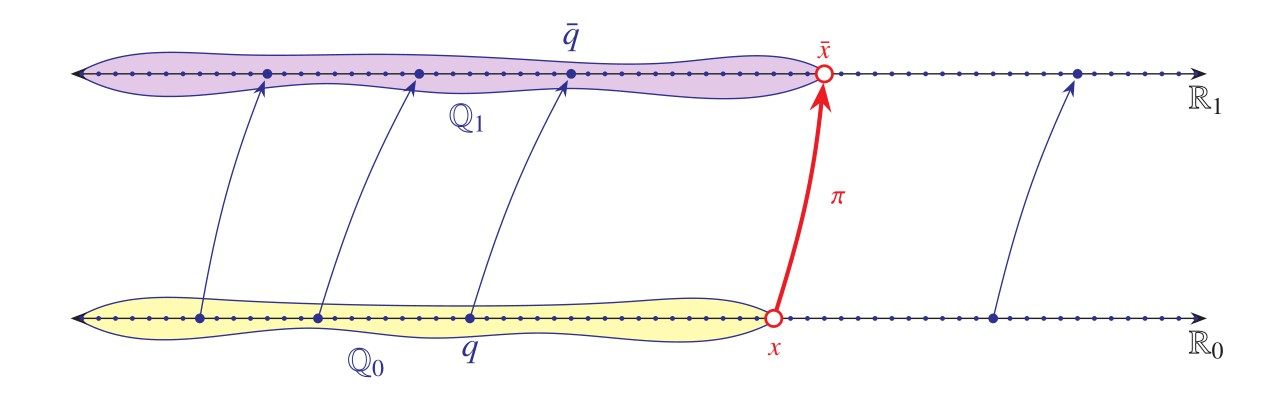
\includegraphics[width=\textwidth]{media/uniqueness-of-the-reals.jpg}
    \vspace{-24pt}
    \caption{An isomorphic mapping $\pi : \RR_0 \to \RR_1$ (courtesy
    of Hamkins \cite{img:uniqueness-of-r}).}
  \end{tightfigure}

  We now extend this isomorphism to the entire fields, $\RR_0$ and
  $\RR_1$, using Dedekind cuts (\defref{dedekind-cuts}). The
  Archimedean property ensures that every element $x$ in $\RR_0$
  defines a unique cut in $\QQ_0$, dividing it into two sets: Those
  rational elements less than $x$ (shown in yellow), and those
  greater than or equal to $x$. Since we have an isomorphism between
  $\QQ_0$ and $\QQ_1$, this cut in $\QQ_0$ corresponds to a similar
  division in $\QQ_1$. By the completeness of $\RR_1$, there must be
  a unique element $\overline{x} \in \RR_1$ that makes this exact
  same cut in $\QQ_1$ (shown in violet). This defines our mapping
  $\pi : x \mapsto \overline{x}$ from $\RR_0$ to $\RR_1$.

  Finally, we verify that the mapping $\pi$ is indeed a field isomorphism:
  \begin{enumerate}
    \item Surjection: Every $y \in \RR_1$ determines a cut in
      $\QQ_1$. By the isomorphism between $\QQ_0$ and $\QQ_1$, this
      corresponds to a cut in $\QQ_0$. By the completeness of
      $\RR_0$, there exists an $x \in \RR_0$ that defines this cut.
      Thus, $\pi(x) = y$.
    \item Injection: If two elements $x_1, x_2 \in \RR_0$ determine
      the same cut in $\QQ_0$, then $x_1 = x_2$ (by the definition of
      Dedekind cuts). Thus, if $\pi(x_1) = \pi(x_2)$, then $x_1$ and
      $x_2$ must define the same cut in $\QQ_0$, which means $x_1 = x_2$.
    \item Field homomorphism: The mapping $\pi$ preserves field
      operations (i.e. addition, multiplication, and order) because
      it is constructed as a continuous extension of the isomorphism
      between the rational subfields $\QQ_0$ and $\QQ_1$.
  \end{enumerate}
  This completes the proof.
\end{proofsketch}

\begin{corollary}[Existence and uniqueness of $\RR$]
  There exists a unique complete ordered field. We call this field
  \textit{the real numbers} $\RR$.
\end{corollary}

\begin{proposition}[Axioms of $\RR$]
  The set $\RR$ has two binary operations, addition ($+$) and
  multiplication ($\cdot$), and is the unique set satisfying the
  following axioms.
  \begin{itemize}
    \item \textbf{Axiom 1 (Commutative Law).} If $a, b \in \RR$, then
      $a + b = b + a$ and $a \cdot b = b \cdot a$.
    \item \textbf{Axiom 2 (Distributive Law).} If $a, b \in \RR$, $a
      \cdot (b + c) = a \cdot b + a \cdot c$.
    \item \textbf{Axiom 3 (Associative Law).} If $a, b \in \RR$, then
      $(a + b) + c = a + (b + c)$ and $(a \cdot b) \cdot c = a \cdot
      (b \cdot c)$.
    \item \textbf{Axiom 4 (Identity Law).} There are special elements
      $\zero, \one \in \RR$, where $a + \zero = a$ and $a \cdot \one
      = a$ for all $a \in \RR$.
    \item \textbf{Axiom 5 (Inverse Law).} For each $a \in \RR$, there
      is an element $-a \in \RR$ such that $a + (-a) = \zero$. If $a
      \neq \zero$, then there is also an element $a^{-\one} \in \RR$
      such that $a \times a^{-\one} = \one$.
    \item \textbf{Axiom 6 (Order Axiom).} There is a nonempty subset
      $P \subseteq \RR$, called the \textit{positive elements}, such that
      \begin{enumerate}
        \item If $a, b \in P$, then $a + b \in P$ and $a \cdot b \in P$;
        \item If $a \in \RR$ and $a \neq \zero$, then either $a \in
          P$ or $-a \in P$, but not both.
      \end{enumerate}
    \item \textbf{Axiom 7 (Completeness Axiom).} Given any nonempty
      $A \subseteq \RR$ where $A$ is bounded above, $A$ has a least
      upper bound. In other words, $\sup(A) \in \RR$ for every such $A$.
  \end{itemize}
\end{proposition}

\begin{proposition}[Suprema are unique]
  If the supremum or infimum of $A \subseteq \RR$ exists, then it is unique.
\end{proposition}

We will only prove that suprema are unique. The infima case is analogous.

\begin{proof}
  Assume for a contradiction that $\alpha$ and $\beta$ are distinct
  least upper bounds of $A$. In particular, both are upper bounds of
  $A$, while $\alpha \neq \beta$. One one hand, since $\alpha$ is a
  least upper bound and $\beta$ is an upper bound, we must have
  $\alpha \leq \beta$. On the other hand, since $\beta$ is a least
  upper bound and $\alpha$ is an upper bound, we must have $\beta
  \leq \alpha$. In summary,
  \[ \alpha \leq \beta \qquad \text{and} \qquad \beta \leq \alpha. \]
  This implies that $\alpha = \beta$, giving our contradiction.
\end{proof}

\begin{theorem}[Square roots exist]
  If $a \in \RR$ and $a \geq 0$, then $\sqrt{a} \in \RR$.
\end{theorem}

\begin{proofidea}
  One can show that $\sqrt{a} = \sup(\set{x \in \RR : x^2 < a})$,
  which is in $\RR$ by completeness.
\end{proofidea}

\begin{theorem}[Suprema analytically]
  \thmlabel{suprema-analytically}
  Let $A \subseteq \RR$. Then $\sup(A) = \alpha$ if and only if
  \begin{enumerate}
    \item $\alpha$ is an upper bound of $A$, and
    \item Given any $\epsilon > 0$, $\alpha - \epsilon$ is
      \textit{not} an upper bound of $A$. That is, there is some $x
      \in A$ for which $x > \alpha - \epsilon$.
  \end{enumerate}
  Likewise, $\inf(A) = \beta$ if and only if
  \begin{enumerate}
    \item $\beta$ is a lower bound of $A$, and
    \item Given any $\epsilon > 0$, $\beta + \epsilon$ is
      \textit{not} a lower bound of $A$. That is, there is some $x
      \in A$ for which $x < \beta + \epsilon$.
  \end{enumerate}
\end{theorem}

We will only prove the suprema case. The infima case is analogous.

\begin{proof}
  \phantom{.}

  $(\Rightarrow)$ First, assume that $\sup(A) = \alpha$. We aim to
  prove part 1 and 2. The first of these is immediate: Since $\sup(A)
  = \alpha$, $\alpha$ is the least upper bound of $A$, which of
  course also implies that it is an upper bound of $A$.

  Now we will show part 2. Let $\epsilon > 0$, Since $\alpha -
  \epsilon < \alpha$, we know that $\alpha - \epsilon$ is not an
  upper bound of $A$, because if so that would contradict $\alpha$
  being the least upper bound of $A$. And so, since $\alpha -
  \epsilon$ is not an upper bound, there must be some $x$ who is
  greater than $\alpha - \epsilon$.

  $(\Leftarrow)$ Now assume part 1 and 2. We aim to prove that
  $\sup(A) = \alpha$. That is, we wish to show that $\alpha$ is an
  upper bound of $A$ (which is implied directly by part 1), and for
  any other upper bound $\beta$, we have $\alpha \leq \beta$. We have
  only the latter to prove. Assume that $\beta$ is some other upper
  bound of $A$, and assume for a contradiction that $\beta < \alpha$.
  Note that $0 < \alpha - \beta$. We will use $(\alpha - \beta)$ as
  our $\epsilon$, and then apply part 2 to contradict $\beta$ being
  an upper bound.

  Now we will work it out formally. Let $\epsilon = \alpha - \beta$.
  Since $\epsilon > 0$, by part 2 there exists some $x \in A$ such
  that $x > \alpha - \epsilon = \alpha - (\alpha - \beta) = \beta$.
  But this is a contradiction, because we assumed that $\beta$ was an
  upper bound of $A$, and yet we found another element $x \in A$ that
  is larger than $\beta$.
\end{proof}

\begin{remark}
  Note that the forward direction of the proof also works well by
  contrapositive. The contrapositive of
  \begin{center}
    $\sup(A) = \alpha$ $\implies$ For all $\epsilon > 0$ there is an
    $x \in A$ such that $x > \alpha - \epsilon$ \\
    \raggedright is \par
    \centering There is an $\epsilon > 0$ such that for all $x \in A$
    we have $x \leq \alpha - \epsilon$ $\implies$ $\sup(A) \neq \alpha$.
  \end{center}
  And to prove this, just observe that the left-hand side implies
  that $\alpha - \epsilon$ is an upper bound of $A$, and so $\sup(A)
  \leq \alpha - \epsilon$, which of course implies that $\sup(A) \neq
  \alpha$, as desired.
\end{remark}

\begin{lemma}[The Archimedean principle]
  \lemlabel{archimedean-principle}
  If $a$ and $b$ are real numbers with $a > 0$, then there exists a
  natural number $n$ such that $na > b$.

  In particular, for any $\epsilon > 0$ there exists $n \in \NN$ such
  that $\frac{1}{n} < \epsilon$.
\end{lemma}

\begin{proof}
  We aim to show that $na > b$ for some $n \in \NN$; by dividing over
  the $a$, we aim to prove that there is some $n \in \NN$ such that
  $n > b/a$. Now, the number $b/a$ is just some real number that we
  know nothing about. In fact, let's just call it $x$. So,
  equivalently, we are trying to prove that given any real number
  $x$, there is some integer $n$ such that $n > x$.

  Assume for a contradiction that there is no integer larger than
  $x$. That is, assume that $x$ is an upper bound on the set $\NN$.
  Then $\NN$ is a subset of $\RR$ that is bounded above, and so by
  the completeness of $\RR$ we deduce that $\sup(\NN)$ exists. Call
  this supremum $\alpha$. Since $\alpha$ is the least upper bound of
  $\NN$, we know that $\alpha - 1$ is not an upper bound. That is,
  there exists some integer $m > \alpha - 1$. Adding 1 to each side,
  \[ m + 1 > \alpha. \]
  But this is a contradiction. If $\alpha$ is the supremum of $\NN$,
  then it is an upper bound on $\NN$. But we found $(m + 1) \in \NN$
  which is larger than $\alpha$. This concludes the first statement
  in the principle.

  The second part follows directly from the first by letting $a =
  \epsilon$ and $b = 1$, and dividing over the $n$.
\end{proof}

\begin{example}
  Show that $\inf(\set{\frac{1}{n} : n \in \NN}) = 0$.
  \begin{proof}
    Let $A = \set{\frac{1}{n} : n \in \NN}$. We will use the analytic
    definition of suprema (\thmref{suprema-analytically}). We must
    then show that 0 is a lower bound of $A$ and that, for all
    $\epsilon > 0$, $0 + \epsilon$ is not a lower bound of $A$.

    The first of these is almost immediate: Since 1 and $n$ are
    positive for each $n \in \NN$, so is $1/n$. So $1/n > 0$, and
    thus 0 is indeed a lower bound for $A$.

    Working toward the second, let $\epsilon > 0$. Then by the
    Archimedean principle (\lemref{archimedean-principle}), there
    exists some $n \in \NN$ such that $\frac{1}{n} < \epsilon$. This
    element, $\frac{1}{n}$, is in $A$ and is less than $0 +
    \epsilon$. So $0 + \epsilon$ is not a lower bound of $A$.
  \end{proof}
\end{example}

\begin{example}
  Show that $\sup(\set{\frac{1}{n} : n \in \NN}) = 1$.
  \begin{proof}
    Let $A = \set{\frac{1}{n} : n \in \NN}$. We will use the analytic
    definition of suprema (\thmref{suprema-analytically}). We must
    then show that 1 is an upper bound of $A$ and that, for all
    $\epsilon > 0$, $1 - \epsilon$ is not an upper bound of $A$.

    For the first of these, note that since $n \geq 1$ for all $n \in
    \NN$, and by dividing over the $n$ we have that $1 \geq
    \frac{1}{n}$ for all $n \in \NN$. So 1 is indeed an upper bound for $A$.

    Working towards the second, let $\epsilon > 0$. We need to show
    that there is some $x \in A$ such that $1 - \epsilon < x$. But
    this is always accomplished by the number 1: Clearly $1 \in A$
    and $1 - \epsilon < 1$.
  \end{proof}
\end{example}

\begin{definition}[Density]
  Suppose $A$ and $B$ are ordered field. Then $A$ is \vocab{dense} in
  $B$ if, for any $x, y \in B$, there exists $a \in A$ such that $x < a < y$.
\end{definition}

\begin{example}
  The propositions below are left without proof.
  \begin{itemize}
    \item $\QQ$ is dense in $\QQ$.
    \item $\RR \setminus \QQ$ is dense in $\QQ$.
    \item $\ZZ$ is \textit{not} dense in $\QQ$.
  \end{itemize}
\end{example}

\begin{lemma}
  \lemlabel{precursor-to-q-is-dense-in-r}
  Let $x, y \in \RR$. If $y - x > 1$, then there exists $z \in \ZZ$
  such that $x < z < y$.
\end{lemma}

\begin{proof}
  First assume that $x$ and $y$ are at least 0, and consider the set
  \[ A = \set{n \in \NN_0 : n \leq x}. \]
  Since $x \geq 0$, this set is non-empty, and since it is a set of
  nonnegative integers which is bounded above by $x$, this set is
  finite. By induction on the size of $A$, we can show that $\max(A)$
  exists and is an element of $A$. Call this maximum $M$. We claim $z
  := M + 1$ works.

  Note that since $M \in \NN_0$, also $z \in \NN_0$. Furthermore,
  since $z$ is larger than the largest element of $A$, $z$ is not in
  $A$, implying that $x < z$. Finally,
  \[ M \leq x \qquad \text{implies that} \qquad M + 1 \leq x + 1 \leq y. \]
  So $z < y$. In summary, we have shown that $x < z < y$, as desired.

  The cases where $x$ and $y$ are not at least 0 are similar. If both
  are negative, then by considering $-x$ and $-y$ the above argument
  gives an integer $z$ where $-y < z < -x$, showing that $-z$ works,
  since $x < -z < y$. If one is positive and one is negative, then 0 works.
\end{proof}

\begin{theorem}[$\QQ$ is dense in $\RR$]
  \thmlabel{q-is-dense-in-r}
  The rational numbers are dense in the real numbers.
\end{theorem}

\begin{proof}
  Pick any $x, y \in \RR$ where $x < y$. We need to show that there
  exists some $\frac{m}{n} \in \QQ$ (with $m, n \in \ZZ$) such that
  \[ x < \frac{m}{n} < y. \]
  First note that if $x < 0 < y$ then we are done, since $0 \in \QQ$.
  Furthermore, if we can show that the theorem holds for the case
  that $x$ and $y$ are positive, then it holds when they are negative
  ($0 < x < \frac{m}{n} < y$ implies $-y < \frac{-m}{n} < -x < 0$),
  so we may assume $x$ and $y$ are positive.

  Since $y - x > 0$, by the Archimedean principle
  (\lemref{archimedean-principle}) there exists some $n \in \NN$ such
  that $n (y - x) > 1$; i.e. $ny - nx > 1$. And so, by
  \lemref{precursor-to-q-is-dense-in-r}, there is some integer $m$ with
  \[ nx < m < ny. \]
  That is,
  \[ x < \frac{m}{n} < y, \]
  which concludes the proof.
\end{proof}

\begin{remark}
  The proof of \lemref{precursor-to-q-is-dense-in-r} also implies
  that, for any $x \in \RR$, there exists an integer $M$ such that $M
  \leq x \leq M + 1$. In particular, it implies that the floor and
  ceiling functions exist.
\end{remark}

\begin{definition}[Ceiling and floor functions]
  Let $x \in R$.
  \begin{itemize}
    \item The \textit{ceiling} of $x$, denoted $\ceil{x}$, is the
      integer $n$ such that $x \leq n < x + 1$.
    \item The \textit{floor} of $x$, denoted $\floor{x}$, is the
      integer $n$ such that $x  - 1 < n \leq x$.
  \end{itemize}
\end{definition}

\begin{definition}[Closed and open intervals]
  Define the \textit{closed interval} $[a, b]$ to be $\set{x \in \RR
  : a \leq x \leq b}$. Likewise the \textit{open interval} $(a, b)$
  is defined to be $\set{x \in \RR : a < x < b}$, and half-open
  intervals and intervals to $\pm\infty$ are again exactly as you would expect.
\end{definition}

\begin{theorem}[Characterization of intervals]
  Let $S$ be a subset of $\RR$ that contains at least two points. If
  $S$ has the property such that
  \[ \text{if $x, y \in S$ and $x < y$, then $[x, y] \subseteq S$}, \tag{1} \]
  then $S$ is an interval.
\end{theorem}

\begin{proof}
  There are four cases to consider: (1) $S$ is bounded, (2) $S$ is
  bounded above but not below, (3) $S$ is bounded below but not
  above, and (4) $S$ is neither bounded above nor below.

  \textbf{Case (1).} Let $a = \inf(S)$ and $b = \sup(S)$. Then $S
  \subseteq [a, b]$ and we will show that $(a, b) \subseteq S$. If $a
  < z < b$, then $z$ is not a lower bound of $S$, so there exists $x
  \in S$ with $x < z$. Also, $z$ is not an upper bound of $S$, so
  there exists $y \in S$ with $z < y$. Therefore, $z \in [x, y]$, so
  property (1) implies that $z \in S$. Since $z$ is an arbitrary
  element of $(a, b)$, we conclude that $(a, b) \subseteq S$. Now if
  $a \in S$ and $b \in S$, then $S = [a, b]$. If $a \notin S$ and $b
  \notin S$, then $S = (a, b)$. The other possibilities lead to
  either $S = (a, b]$ or $S = [a, b)$.

  \textbf{Case (2).} Let $b = \sup(S)$. Then $S \subseteq (-\infty,
  b]$ and we will show that $(-\infty, b) \subseteq S$. If $z < b$,
  then $z$ is not an upper bound of $S$, so there exists $y \in S$
  with $z < y$. Also, since $S$ is not bounded below, there exists $x
  \in S$ with $x < z$. By property 1, $z \in [x, y] \subseteq S$.
  Since $z$ is an arbitrary element of $(-\infty, b)$, we conclude
  that $(-\infty, b) \subseteq S$. Now if $b \in S$, then $S =
  (-\infty, b]$, and if $b \notin S$, then $S = (-\infty, b)$.

  \textbf{Case (3).} Let $a = \inf(S)$. Then $S \subseteq [a,
  \infty)$ and we will show that $(a, \infty) \subseteq S$. If $a <
  z$, then $z$ is not a lower bound of $S$, so there exists $x \in S$
  with $x < z$. Also, since $S$ is not bounded above, there exists $y
  \in S$ with $z < y$. By property 1, $z \in [x, y] \subseteq S$.
  Since $z$ is an arbitrary element of $(a, \infty)$, we conclude
  that $(a, \infty) \subseteq S$. Now if $a \in S$, then $S = [a,
  \infty]$, and if $a \notin S$, then $S = (a, \infty)$.

  \textbf{Case (4).} We will show that $S = (-\infty, \infty)$. Pick
  any $x, y \in S$ with $x < y$, property 1 implies that $[x, y]
  \subseteq S$. Since $S$ is neither bounded above nor below, and the
  choice of $x$, $y$ is arbitrary, we conclude that $(-\infty,
  \infty) \subseteq S$. Also, every subset of $\RR$ is a subset of
  $(-\infty, \infty)$, thus $S = (-\infty, \infty)$.
\end{proof}

\begin{theorem}[The nested intervals property]
  \thmlabel{nested-intervals-property}
  For each $n \in \NN$, assume we are given a closed interval $I_n =
  [a_n, b_n]$. Also, assume that each $I_n$ contains $I_{n + 1}$.
  Then, the resulting nested sequence of closed intervals
  \begin{align*}
    I_1 \supseteq I_2 \supseteq I_3 \supseteq I_4 \supseteq \dots
  \end{align*}
  has a nonempty intersection. That is,
  \begin{align*}
    \bigcap_{n = 1}^{\infty} I_n \neq \emptyset.
  \end{align*}
\end{theorem}

\begin{proof}
  In order to show that $\bigcap_{n = 1}^{\infty} I_n \neq \emptyset$
  is not empty, we are going to use the completeness axiom to produce
  a single real number $x$ satisfying $x \in I_n$ for every $n \in
  \NN$. Now, the completeness axiom is a statement about bounded
  sets, and the one we want to consider is the set
  \[ A = \set{a_n : n \in \NN} \]
  of left-hand endpoints of the interval. Because the intervals are
  nested, we see that every $b_n$ serves as an upper bound for $A$.
  Thus, we are justified in setting
  \[ x = \sup(A). \]
  Now, consider a particular $I_n = [a_n, b_b]$. Because $x$ is an
  upper bound for $A$, we have $a_n \leq x$. The fact that each $b_n$
  is an upper bound for $A$ and that $x$ is the least upper bound
  implies $x \leq b_n$.

  Altogether then, we have $a_n \leq x \leq b_n$, which means $x \in
  I_n$ for every choice of $n \in \NN$. Hence, $x \in \bigcap_{n =
  1}^{\infty} I_n$, and the intersection is not empty.
\end{proof}

\begin{remark}
  Note that the conclusion of \thmref{nested-intervals-property} need
  not hold if each $I_n$ is allowed to be an open interval.
\end{remark}

\setchapterpreamble{\dictum[David Hilbert, \textit{Über das
  Unendliche}]{``No one shall expel us from the paradise that Cantor
has created.''}}
\chapter{Cardinality}
\begin{definition}[Cardinality]
  \deflabel{cardinality-bijection}
  Let $S$ and $T$ be sets. Then, $\abs{S} = \abs{T}$ if and only if
  there is a bijection from $S$ to $T$.
\end{definition}

\begin{definition}[Cardinality cont.]
  \deflabel{cardinality-injection}
  $\abs{S} \leq \abs{T}$ if and only if there is an injection from $S$ to $T$.
\end{definition}

\begin{remark}
  Our definitions above introduce two fundamental relations on
  cardinality, i.e. $\size{S} = \size{T}$ and $\size{S} \leq
  \size{T}$. We need to make sure that these relations have the
  mathematical properties we expect them to have. That is, we want
  $\size{S} = \size{T}$ to be an equivalence relation and $\size{S}
  \leq \size{T}$ to be a partial order.

  For the relation $\size{S} = \size{T}$, it's easy to show that it
  defines an equivalence relation:
  \begin{itemize}
    \item Reflexivity: Every set has a bijection with itself, i.e.
      $\size{S} = \size{S}$.
    \item Symmetry: If there is a bijection $f$ from $S$ to $T$, then
      $f^{-1}$ is a bijection from $T$ to $S$, and thus $\size{T} = \size{S}$.
    \item Transitivity: If there are bijections $f$ from $S$ to $T$
      and $g$ from $T$ to $U$, then their composition $h = g \circ f$
      is a bijection from $S$ to $U$. Hence, $\size{S} = \size{U}$.
  \end{itemize}

  For the relation $\size{S} \leq \size{T}$, we must establish that
  it's a partial order:
  \begin{itemize}
    \item Reflexivity: Every set has an injection to itself, i.e.
      $\size{S} \leq \size{S}$.
    \item Transitivity: If there exist injections $f$ from $S$ to $T$
      and $g$ from $T$ to $U$, then their composition $h = g \circ f$
      is an injection from $S$ to $U$. Hence, $\size{S} \leq \size{U}$.
  \end{itemize}

  The remaining property, antisymmetry, is where things get
  interesting, since it's not immediately obvious. Antisymmetry means
  that if $\size{S} \leq \size{T}$ and $\size{T} \leq \size{S}$, then
  $\size{S} = \size{T}$. Using our definition, this translates to: If
  there is an injection from $S$ to $T$ and an injection from $T$ to
  $S$, then there should be a bijection between $S$ and $T$. This is
  exactly what the Schröder-Bernstein theorem
  (\thmref{schröder-bernstein}) guarantees.
\end{remark}

\begin{theorem}[Schröder-Bernstein theorem]
  \thmlabel{schröder-bernstein}
  If there exist injections $f : A \to B$ and $g : B \to A$ between
  the sets $A$ and $B$, then there exists a bijection $h : A \to B$.

  In terms of the cardinality of the two sets, this implies that if
  $\size{A} \leq \size{B}$ and $\size{B} \leq \size{A}$, then
  $\size{A} = \size{B}$.
\end{theorem}

\begin{proof}
  The strategy is to partition $A$ and $B$ into components
  \[ A = X \cup X' \qquad \text{and} \qquad B = Y \cup Y' \]
  with $X \cap X' = \emptyset$ and $Y \cap Y' = \emptyset$, in such a
  way that $f$ is a surjection from $X$ to $Y$, and $g$ is a
  surjection from $Y'$ to $X'$. Achieving this would lead to a proof
  that there is a bijection $h$ from $A$ to $B$. Why? For all $x \in
  X'$, there exists a unique $y \in Y'$ satisfying $g(y) = x$. This
  means that there is a well-defined inverse function $g^{-1}(x) = y$
  that maps $X'$ to $Y'$. Setting
  \begin{align*}
    h(x) =
    \begin{cases}
      f(x) & \text{if $x \in X$} \\
      g^{-1}(x) & \text{if $x \in X'$}
    \end{cases}
  \end{align*}
  gives the desired bijection from $A$ to $B$.

  Now, let $X_1 = A \setminus g(B)$ and inductively define a sequence
  of sets by letting $X_{n + 1} = g(f(X_n))$. We show that $\set{X_n
  : n \in \NN}$ is a pairwise disjoint collection of subsets of $A$,
  while $\set{f(X_n) : n \in \NN}$ is a similar collection in $B$.

  To see that the sets $X_1, X_2, X_3, \dots$ are pairwise disjoint,
  note that $X_1 \cap X_n = \emptyset$ for all $n \geq 2$ because
  $X_1 = A \setminus g(B)$ and $X_n \subseteq g(B)$. (Why? $f$ is a
    mapping from $A$ to $B$, so we have that $f(X_n) \subseteq B$, and
  thus $X_{n + 1} = g(f(X_n)) \subseteq g(B)$.) In the general case
  of $X_n \cap X_m$ where $1 < n < m$, note that if $x \in X_n \cap
  X_m$ then $f^{-1}(g^{-1}(x)) \in X_{n - 1} \cap X_{m - 1}$.
  Continuing in this way, we can show $X_1 \cap X_{m - n + 1}$ is not
  empty, which is a contradiction. Thus $X_n \cap X_m = \emptyset$.
  Just to be clear, the disjointness of the $X_n$ sets is not crucial
  to the overall proof, but it does help paint a clearer picture of
  how the sets $X$ and $X'$ are constructed.

  Let $X = \bigcup_{n = 1}^{\infty} X_n$ and $Y = \bigcup_{n =
  1}^{\infty} f(X_n)$. We show that $f$ is a surjection from $X$ to
  $Y$. This is straightforward. Each $x \in X$ comes from some $X_n$
  and so $f(x) \in f(X_n) \subseteq Y$. Likewise, each $y \in Y$ is
  an element of some $f(X_n)$ and thus $y = f(x)$ for some $x \in X_n
  \subseteq X$. Thus $f : A \to B$ is a surjection.

  Let $X' = A \setminus X$ and $Y' = B \setminus Y$. Let $y \in Y'$.
  Then $y \notin f(X_n)$ for all $n$ (by definition of $Y'$). We also
  conclude that $g(y) \notin X_{n + 1}$ for all $n$. (Why? Suppose if
    $g(y) \in X_{n + 1}$ for some $n$, then $g(y) \in g(f(X_n))$. That
    is, $g(y) = g(z)$ for some $z \in f(X_n)$, and since $g$ is
    injective, we have $y = z$ and thus $y \in f(X_n)$, which is a
  contradiction.) Clearly, $g(y) \notin X_1$ either (because $g(y)
  \subseteq g(B)$ and $X_1 = A \setminus g(B)$) and so $g$ is a
  mapping from $Y'$ to $X'$. To see that $g$ is a surjection from
  $Y'$ to $X'$, let $x \in X'$ be arbitrary. Because $X' \subseteq
  g(Y') \subseteq g(B)$, there exists $y \in B$ with $g(y) = x$.
  Could $y$ be an element of $Y$? No, because if $y \in Y$, $g(y)$
  would be in $g(Y)$, and since $g(Y) \subseteq X$ (by definition of
  $Y$), this would mean $g(y) \in X$. But we're considering an $x \in
  X'$ with $g(y) = x$, so this is a contradiction as $X \cap X' =
  \emptyset$. Hence $y \in Y'$ and $g : Y' \to X'$ is a surjection.
\end{proof}

\begin{definition}[Cardinality cont.]
  \deflabel{cardinality-surjection}
  $\size{S} \geq \size{T}$ if and only if there is a surjection from $S$ to $T$.
\end{definition}

\begin{remark}
  Again, we must establish that $\size{S} \geq \size{T}$ defines a
  partial order. Reflexivity and transitivity are obvious. Now we
  will show antisymmetry. Suppose $\size{S} \geq \size{T}$ and
  $\size{T} \geq \size{S}$. Then, by definition, there are
  surjections from $S$ to $T$ and from $T$ to $S$. Using the axiom of
  choice, one can prove that there exists a surjection from $X$ to
  $Y$ if and only if there exists an injection from $Y$ to $X$. We
  conclude that $\size{T} \leq \size{S}$ and $\size{S} \leq
  \size{T}$, which implies $\size{S} = \size{T}$ by \thmref{schröder-bernstein}.
\end{remark}

\begin{theorem}[$\abs{\ZZ} = \abs{\NN}$]
  \thmlabel{cardinality-of-z-equal-n}
  There are as many integers as there are natural numbers.
\end{theorem}

\begin{proof}
  Define the function $f : \NN \to \ZZ$ with
  \begin{align*}
    f(n) =
    \begin{cases}
      (n - 1) / 2 & \text{if $n$ is odd} \\
      - n / 2 & \text{if $n$ is even}.
    \end{cases}
  \end{align*}
  Clearly, $f$ is a bijection. (See the following diagram.)

  \begin{tightfigure}
    \centering
    \begin{tikzpicture}[baseline]
      % Set up a matrix for the main content
      \matrix (m) [matrix of math nodes,
        column sep=0.25cm,
      row sep=0cm] {
        \NN : & 1 & 2 & 3 & 4 & 5 & 6 & 7 & \cdots \\
        & \updownarrow & \updownarrow & \updownarrow & \updownarrow &
        \updownarrow & \updownarrow & \updownarrow & \\
        \ZZ : & 0 & -1 & 1 & -2 & 2 & -3 & 3 & \cdots \\
      };
    \end{tikzpicture}
  \end{tightfigure}

  Hence, by \defref{cardinality-bijection}, $\size{\NN} = \size{\ZZ}$.
\end{proof}

\begin{remark}
  \thmref{cardinality-of-z-equal-n} also shows that two sets can have
  the same cardinality even if one is a proper subset of the other
  and the ``larger'' one even has infinitely many more elements than
  the ``smaller'' one. Make sure you take a moment to appreciate how
  remarkably, wonderfully weird this is.
\end{remark}

\begin{theorem}[$\abs{\QQ} = \abs{\NN}$]
  \thmlabel{cardinality-of-q-equal-n}
  There are as many rational numbers as there are natural numbers.
\end{theorem}

\begin{proof}
  Let $A_1 = \set{0}$ and for each $n \geq 2$, let $A_n$ be the set given by
  \[ A_n = \set{\pm\frac{p}{q} : \text{where $p, q \in \NN$ are in
  lowest terms with $p + q$ = n}}. \]
  The first few of these sets look like
  \[ A_1 = \set{0}, \qquad A_2 = \left\{\frac{1}{1},
    \frac{-1}{1}\right\}, \qquad A_3 = \left\{\frac{1}{2},
  \frac{-1}{2}, \frac{2}{1}, \frac{-2}{1}\right\}, \]
  \[ A_4 = \left\{\frac{1}{3}, \frac{-1}{3}, \frac{3}{1},
    \frac{-3}{1}\right\}, \qquad \text{and} \qquad A_5 =
    \left\{\frac{1}{4}, \frac{-1}{4}, \frac{2}{3}, \frac{-2}{3},
  \frac{3}{2}, \frac{-3}{2}, \frac{4}{1}, \frac{-4}{1}\right\}. \]
  The crucial observation is that each $A_n$ is finite and every
  rational number appears in exactly one of these sets. A bijection
  with $\NN$ is then achieved by consecutively listing the elements
  in each $A_n$.

  \begin{tightfigure}
    \centering
    \usetikzlibrary{decorations.pathreplacing}
    \begin{tikzpicture}[baseline]
      % Set up a matrix for the main content
      \matrix (m) [matrix of math nodes,
        column sep=0.25cm,
      row sep=0cm] {
        \NN : & 1 & 2 & 3 & 4 & 5 & 6 & 7 & 8 & 9 & 10 & 11 & 12 & \cdots \\
        & \updownarrow & \updownarrow & \updownarrow & \updownarrow &
        \updownarrow & \updownarrow & \updownarrow & \updownarrow &
        \updownarrow & \updownarrow & \updownarrow & \updownarrow & \\
        \QQ : &
        \makebox[\widthof{$-\dfrac{1}{1}$}][c]{$\vphantom{\dfrac{1}{1}}0$}
        & \dfrac{1}{1} &
        -\dfrac{1}{1} & \dfrac{1}{2} &
        -\dfrac{1}{2} & \dfrac{2}{1} & -\dfrac{2}{1} & \dfrac{1}{3} &
        -\dfrac{1}{3} & \dfrac{3}{1} & -\dfrac{3}{1} & \dfrac{1}{4} & \cdots \\
      };

      % Draw the underbraces
      \draw [decorate, decoration={brace, amplitude=6pt, mirror, raise=2pt}]
      (m-3-2.south west) -- (m-3-2.south east) node[midway, below=10pt] {$A_1$};

      \draw [decorate, decoration={brace, amplitude=6pt, mirror, raise=2pt}]
      (m-3-3.south west) -- (m-3-4.south east) node[midway, below=10pt] {$A_2$};

      \draw [decorate, decoration={brace, amplitude=6pt, mirror, raise=2pt}]
      (m-3-5.south west) -- (m-3-8.south east) node[midway, below=10pt] {$A_3$};

      \draw [decorate, decoration={brace, amplitude=6pt, mirror, raise=2pt}]
      (m-3-9.south west) -- (m-3-12.south east) node[midway,
      below=10pt] {$A_4$};
    \end{tikzpicture}
  \end{tightfigure}

  Admittedly, writing an explicit formula for this correspondence
  would be an awkward task, and attempting to do so is not the best
  use of time. What matters is that we see why every rational number
  appears in the correspondence exactly once. Given, say, $22/7$, we
  have that $22/7 \in A_{29}$. Because the set of elements in $A_1,
  \dots, A_{28}$ is finite, we can be confident that $22/7$
  eventually gets included in the sequence. The fact that this line
  of reasoning applies to any rational number $p/q$ is our proof that
  the correspondence is surjective. To verify that it is injective,
  we observe that the sets $A_n$ were constructed to be disjoint so
  that no rational number appears twice. This completes the proof.
\end{proof}

\begin{theorem}[$\abs{\RR} > \abs{\NN}$]
  \thmlabel{cardinality-of-r-greater-than-n}
  There are more real numbers than natural numbers.
\end{theorem}

\begin{proof}
  Assume, for the sake of contradiction, that $\size{\RR} =
  \size{\NN}$, which implies that there is a bijection $f : \NN \to
  \RR$. What this suggests is that it is possible to enumerate the
  elements of $\RR$. If we let $x_1 = f(x_1)$, $x_2 = f(x_2)$, and so
  on, then the fact that $f$ is bijective (and thus surjective) means
  that we can write
  \[ \RR = \set{x_1, x_2, x_3, x_4, \dots} \tag{1} \]
  and be confident that every real number appears somewhere on the
  list. We will now use the nested intervals property
  (\thmref{nested-intervals-property}) to produce a real number that
  is not there.

  Let $I_1$ be a closed interval that does not contain $x_1$. Next,
  let $I_2$ be a closed interval, contained in $I_1$, which does not
  contain $x_2$. The existence of such $I_2$ is easy to verify.
  Certainly $I_1$ contains two smaller disjoint closed intervals, and
  $x_2$ can only be in one of these. In general, given an interval
  $I_n$, construct $I_{n + 1}$ to satisfy
  \begin{enumerate}
    \item $I_{n + 1} \subseteq I_n$ and
    \item $x_{n + 1} \notin I_{n + 1}$.
  \end{enumerate}
  We now consider the intersection $\bigcap_{n = 1}^{\infty} I_n$. If
  $x_k$ is some real number from the list in (1), then we have $x_k
  \notin I_k$, and it follows that
  \[ x_k \notin \bigcap_{n = 1}^{\infty} I_n. \]
  Now, we are assuming that the list in (1) contains every real
  number, and this leads to the conclusion that
  \[ \bigcap_{n = 1}^{\infty} I_n = \emptyset. \]
  However, the nested intervals property
  (\thmref{nested-intervals-property}) asserts that $\bigcap_{n =
  1}^{\infty} I_n \neq \emptyset$. So there is at least one $x \in
  \bigcap_{n = 1}^{\infty} I_n$ that, consequently, cannot be on the
  list in (1). This contradiction means that such an enumeration of
  $\RR$ is impossible, and we conclude that $\size{\RR} \neq \size{\NN}$.

  We are not done yet. We still have to show that $\size{\RR} \geq
  \size{\NN}$. This step is straightforward. Define the function $g :
  \RR \to \NN$ with
  \begin{align*}
    g(x) =
    \begin{cases}
      n & \text{if $x = n$ for some $n \in \NN$} \\
      0 & \text{otherwise}.
    \end{cases}
  \end{align*}
  This function maps each real number that is a natural number to
  itself, and all other real numbers to 0. Since every natural number
  is the image of at least one real number under $g$, the function is
  surjective. Therefore, by \defref{cardinality-surjection}, we have
  $\size{\RR} \geq \size{\NN}$. Combining this with our previous
  result that $\size{\RR} \neq \size{\NN}$, we conclude that
  $\size{\RR} > \size{\NN}$.
\end{proof}

\begin{definition}[Countable and uncountable sets]
  \deflabel{countable}
  A set $S$ is \vocab{countable} if
  \begin{enumerate}
    \item its cardinality $\size{S}$ is less than or equal to $\size{\NN}$.
    \item there exists an injection from $S$ to $\NN$.
    \item $S$ is empty or there exists a surjection $\NN$ to $S$.
    \item there exists a bijection from $S$ to a subset of $\NN$.
    \item $S$ is either finite or \textit{countably infinite}.
  \end{enumerate}
  All of the definitions above are equivalent.

  A set $S$ is \vocab{countably infinite} if its cardinality
  $\size{S}$ is exactly $\NN$.

  A set $S$ is \vocab{uncountable} if it is not countable. That is,
  its cardinality $\size{S}$ is greater than $\size{\NN}$.
\end{definition}

\begin{corollary}[$\NN$ is countable]
  The set of natural numbers is countable.
\end{corollary}

\begin{corollary}[$\ZZ$ is countable]
  The set of integers is countable.
\end{corollary}

\begin{corollary}[$\QQ$ is countable]
  \corlabel{q-is-countable}
  The set of rational numbers is countable.
\end{corollary}

\begin{corollary}[$\RR$ is uncountable]
  \corlabel{r-is-uncountable}
  The set of real numbers is uncountable.
\end{corollary}

\begin{theorem}
  An uncountable collection of disjoint open intervals in $\RR$ cannot exist.
\end{theorem}

\begin{proof}
  We use contradiction. Suppose there exists an uncountable
  collection of disjoint open intervals in $\RR$. By the density of
  $\QQ$ in $\RR$ (\thmref{q-is-dense-in-r}), every open interval in
  $\RR$ contains at least one rational number. Therefore, there are
  uncountably many rational numbers. A contradiction of
  \corref{q-is-countable}. Hence, such a collection cannot exist.
\end{proof}

\begin{theorem}[Countable infinity is the smallest infinity]
  \thmlabel{countable-infinity-smallest}
  If $A \subseteq B$ and $B$ is countable, then $A$ is either
  countable or finite.
\end{theorem}

\begin{proof}
  $B$ is a countable set. Thus, there exists a bijection $f : \NN \to
  B$. Let $A \subseteq B$ be an infinite subset of $B$. We show that
  $A$ is countable. Let $n_1 \in \min\set{n \in \NN : f(n) \in A}$.
  As a start to a definition of $g : \NN \to A$, let $g(1) = f(n_1)$.
  Next let $n_2 = \min\set{n \in \NN : f(n) \in A \setminus
  \set{f(n_1)}}$ and let $g(2) = f(n_2)$. We inductively continue
  this process to produce a bijection $g$ from $\NN$ to $A$. In
  general, assume we have defined $g(k)$ for $k < m$, and let $g(m) =
  f(n_m)$ where $n_m = \min\set{n \in \NN : A \setminus \set{f(n_1),
  \dots, f(n_{k - 1})}}$.

  To show that $g$ is injective, observe that $m \neq m'$ implies
  $n_m \neq n_{m'}$ and it follows that $g(m) = f(n_m) \neq f(n_{m'})
  = g(m')$ because $f$ is injective. To show that $g$ is surjective,
  let $a \in A$ be arbitrary. Because $f$ is surjective, $a = f(n')$
  for some $n' \in \NN$. This means $n' \in \set{n : f(n) \in A}$ and
  as we inductively remove the minimal element, $n'$ must eventually
  be the minimum by at least the $(n' -1)$-th step.
\end{proof}

\begin{corollary}[$\size{\NN}$ is the smallest infinity]
  If $A \subseteq \NN$, then either $A$ is finite or $\size{A} = \size{\NN}$.
\end{corollary}

\begin{corollary}[Sizes of infinity]
  There are different sizes of infinity, with countable infinity
  being the smallest. Moreover, $\NN$, $\ZZ$ and $\QQ$ are countable
  while $\RR$ is uncountable.
\end{corollary}

\begin{theorem}[Countable union of countable sets is countable]
  \thmlabel{countable-union-countable}
  A countable union of countable sets is countable. More precisely:
  \begin{enumerate}
    \item If $A_1, A_2, \dots, A_m$ are each countable sets, then
      $A_1 \cup A_2 \cup \dots \cup A_m$ is countable.
    \item If $A_n$ is a countable set for each $n \in \NN$, then the
      set $\bigcup_{n = 1}^{\infty} A_n$ is also countable.
  \end{enumerate}
\end{theorem}

\begin{proof}
  First, we prove part 1 for two countable sets, $A_1$ and $A_2$.
  Some technicalities can be avoided by first replacing $A_2$ with
  the set $B_2 = A_2 \setminus A_1 = \set{x \in A_2 : x \notin A_1}$.
  The point of this is that the union $A_1 \cup B_2$ is equal to $A_1
  \cup A_2$ and the sets $A_1$ and $B_2$ are disjoint.

  Now, because $A_1$ is countable, there exists a bijection $f : \NN
  \to A_1$. If $B_2 = \emptyset$, then $A_1 \cup A_2 = A_1$ which we
  already know to be countable. If $B_2 = \set{b_1, b_2, \dots, b_m}$
  has $m$ elements then define $h : \NN \to A_1 \cup B_2$ via
  \begin{align*}
    h(n) =
    \begin{cases}
      b_n & \text{if $n \leq m$} \\
      f(n - m) & \text{if $n > m$}.
    \end{cases}
  \end{align*}
  The fact that $h$ is bijective follows immediately from the same
  property of $f$. If $B_2$ is infinite, then by
  \thmref{countable-infinity-smallest} it is countable, and so there
  exists a bijection $g : \NN \to B_2$. In this case we define $h :
  \NN \to A_1 \cup B_2$ by
  \begin{align*}
    h(n) =
    \begin{cases}
      f((n + 1) / 2) & \text{if $n$ is odd} \\
      g(n / 2) & \text{if $n$ is even}.
    \end{cases}
  \end{align*}
  Again, the proof that $h$ is bijective is derived directly from the
  fact that $f$ and $g$ are both bijections. Graphically, the
  correspondence takes the form

  \begin{tightfigure}
    \centering
    \begin{tikzpicture}[baseline]
      % Set up a matrix for the main content
      \matrix (m) [matrix of math nodes,
        column sep=0.25cm,
      row sep=0cm] {
        \makebox[\widthof{$A_1 \cup B_2 :$}][r]{$\NN :$} & 1 &
        2 & 3 & 4 & 5 & 6 & \cdots \\
        & \updownarrow & \updownarrow & \updownarrow & \updownarrow &
        \updownarrow & \updownarrow & \\
        A_1 \cup B_2 : & a_1 & b_1 & a_2 & b_2 & a_3 & b_3 & \cdots \\
      };
    \end{tikzpicture}
  \end{tightfigure}

  To prove the more general statement in part 1, we may use
  induction. We have just seen that the result holds for two
  countable sets. Now let's assume that the union of $m$ countable
  sets is countable, and show that the union of $m + 1$ countable
  sets is countable.

  Given $m + 1$ countable sets $A_1, A_2, \dots, A_{m + 1}$, we can write
  \[ A_1 \cup A_2 \cup \dots \cup A_{m + 1} = (A_1 \cup A_2 \cup
  \dots \cup A_m) \cup A_{m + 1}. \]
  Then $C_m = A_1 \cup \dots \cup A_m$ is countable by the induction
  hypothesis, and $C_m \cup A_{n + 1}$ is just the union of two
  countable sets which we know to be countable. This completes the
  proof for part 1.

  For part 2, induction cannot be used because we have an infinite
  number of sets. Instead, we show how arranging $\NN$ into the
  two-dimensional array
  \begin{align*}
    \begin{array}{cccccc}
      1  & 3  & 6  & 10 & 15 & \cdots \\
      2  & 5  & 9  & 14 & \cdots \\
      4  & 8  & 13 & \cdots \\
      7  & 12 & \cdots \\
      11 & \cdots \\
      \vdots \\
    \end{array}
  \end{align*}
  leads to a proof.

  Let's first consider the case where the sets $\set{A_n}$ are
  disjoint. In order to achieve bijection between $\NN$ and
  $\bigcup_{n = 1}^{\infty} A_n$, we first label the elements in each
  countable set $A_n$ as
  \[ A_n = \set{a_{n_1}, a_{n_2}, a_{n_3}, \dots}. \]
  Now arrange the elements of $\bigcup_{n = 1}^{\infty} A_n$ in an
  array similar to the one for $\NN$:
  \begin{align*}
    \begin{array}{cccccccc}
      A_1 & =  & a_{11} & a_{12} & a_{13} & a_{14} & a_{15} & \cdots \\
      A_2 & =  & a_{21} & a_{22} & a_{23} & a_{24} & \cdots &        \\
      A_3 & =  & a_{31} & a_{32} & a_{33} & \cdots &        &        \\
      A_4 & =  & a_{41} & a_{42} & \cdots &        &        &        \\
      A_5 & =  & a_{51} & \cdots &        &        &        &        \\
      & \vdots &        &        &        &        &        &        \\
    \end{array}
  \end{align*}
  This establishes a bijection $g : \NN \to \bigcup_{n = 1}^{\infty}
  A_n$ where $g(n)$ corresponds to the element $a_{jk}$ where $(j,
  k)$ is the row and column location of $n$ in the array for $\NN$.

  If the sets $\set{A_n}$ are not disjoint then our mapping may not
  be injective. In this case we could again replace $A_n$ with $B_n =
  A_n \setminus \set{A_1 \cup \dots \cup A_{n - 1}}$. Another
  approach is to use the previous argument to establish a bijection
  between $\bigcup_{n = 1}^{\infty} A_n$ and an infinite subset of
  $\NN$, and then appeal to \thmref{countable-infinity-smallest}.
  This completes the proof for part 2.
\end{proof}

\begin{theorem}[$\RR \setminus \QQ$ is uncountable]
  There are uncountably many irrational numbers.
\end{theorem}

\begin{proof}
  We use contradiction. Suppose $\RR \setminus \QQ$ is countable. By
  \thmref{countable-union-countable}, we know that a countable union
  of countable sets is countable, thus $(\RR \setminus \QQ) \cup \QQ
  = \RR$ is countable. A contradiction of \corref{r-is-uncountable}.
  Hence, $\RR \setminus \QQ$ is uncountable.
\end{proof}

\begin{theorem}[$\size{\QQ_+} = \size{\NN}$]
  There are as many positive rational numbers as there are natural numbers.
\end{theorem}

\begin{proof}
  The following diagram arranges the rational numbers (with some
  repetition) and illustrates our bijection, which we call the
  \textit{winding bijection}.

  \begin{tightfigure}
    \centering
    \usetikzlibrary{matrix, arrows.meta}
    \begin{tikzpicture}
      % Define the column and row headers
      \foreach \x in {1,...,8} {
        \node at (\x,0.5) {$\x$};
        \node at (-0.5,-\x) {$\x$};
      }
      \node at (9,0.5) {$\cdots$};
      \node at (-0.5,-9) {$\vdots$};

      % Draw horizontal line beneath the column headers
      \draw (0,0) -- (10,0);

      % Draw vertical line to the right of row headers
      \draw (0,0) -- (0,-10);

      % Create the matrix of fractions
      \foreach \x in {1,...,8} {
        \foreach \y in {1,...,8} {
          \node at (\x,-\y) {$\x/\y$};
        }
      }

      % Draw ellipsis
      \foreach \x in {1,...,8} {
        \node at (\x,-9) {$\vdots$};
      }
      \foreach \y in {1,...,8} {
        \node at (9,-\y) {$\cdots$};
      }
      \node at (9,-9) {$\ddots$};

      % To prevent arrows from touching the numbers
      \def\eps{0.25}

      % Draw the arrows
      \foreach \x in {1,...,7} {
        \foreach \y in {2,...,8} {
          \pgfmathparse{int(\x+\y)}
          \ifnum\pgfmathresult<12
          \pgfmathparse{int(mod(\pgfmathresult,2))}
          \ifnum\pgfmathresult=0
          % Diagonal arrows (upward)
          \draw[->,red,thick] (\x+\eps,-\y+\eps) -- (\x+1-\eps,-\y+1-\eps);
          \else
          % Diagonal arrows (downward)
          \draw[->,red,thick] (\x+1-\eps,-\y+1-\eps) -- (\x+\eps,-\y+\eps);
          \fi
          \fi
        }
      }

      % Draw curved arrows
      \foreach \x in {1,...,7} {
        \pgfmathparse{int(mod(\x,2))}
        \ifnum\pgfmathresult=1
        \draw[->,red,thick,bend left=30] (\x+\eps,-1+\eps) to
        (\x+1-\eps,-1+\eps);
        \fi
      }
      \foreach \y in {1,...,7} {
        \pgfmathparse{int(mod(\y,2))}
        \ifnum\pgfmathresult=0
        \draw[->,red,thick,bend right=30] (1-\eps,-\y-\eps) to
        (1-\eps,-\y-1+\eps);
        \fi
      }

      % Draw dashed arrows
      \draw[->,red,thick,dashed] (8+\eps,-2+\eps) to (9-\eps,-1-\eps);
      \draw[->,red,thick,dashed] (9-\eps,-2-\eps) to (8+\eps,-3+\eps);
      \draw[->,red,thick,dashed,bend right=30] (1-\eps,-8-\eps) to
      (1-\eps,-9+\eps);
      \draw[->,red,thick,dashed] (1+\eps,-9+\eps) to (2-\eps,-8-\eps);
      \draw[->,red,thick,dashed] (3-\eps,-8-\eps) to (2+\eps,-9+\eps);
    \end{tikzpicture}
  \end{tightfigure}

  Weaving through this chart, you are guaranteed to hit every
  positive rational number. So if you pair up 1 with the first number
  you hit, 2 with the second number you hit, 3 with the third, and so
  on, then every positive rational number is in a pair. Now, there's
  just one small problem: each rational number is actually hit more
  than once. The number $p/q$ will be written in positions $(p, q),
  (2p, 2q), (3p, 3q), \dots$. But the fix is easy: When you come
  across a number that has already been hit, just skip it. Clearly
  you won't run out of rational numbers, so this does indeed pair up
  everything. So
  \[ f(n) = \text{the $n$th new rational number you reach}. \]
  And that's it.
\end{proof}

\begin{theorem}[$\size{(0, 1)} > \size{\NN}$]
  \thmlabel{cardinality-of-(0,1)-greater-than-n}
  There are more numbers in the open interval $(0, 1)$ than there are
  natural numbers.
\end{theorem}

We will demonstrate a clever argument known as \textit{Cantor's
diagonal argument}.

\begin{proof}
  We proceed by contradiction and assume that there does exist a
  function $f : \NN \to (0, 1)$ that is bijective. For each $m \in
  \NN$, $f(m)$ is a real number between 0 and 1, and we represent it
  using the decimal notation
  \[ f(m) = .a_{m1}a_{m2}a_{m3}a_{m4}a_{m5}\dots. \]
  What is meant here is that for each $m, n \in \NN$, $a_{mn}$ is the
  digit from the set $\set{0, 1, 2, \dots, 9}$ that represents the
  $n$th digit in the decimal expansion of $f(m)$. The bijection
  between $\NN$ and $(0, 1)$ can be summarized in the doubly indexed array
  \begin{align*}
    \begin{array}{ccccccccccc}
      \NN & & (0,1) & & & & & & & & \\
      \hline
      1 & \longleftrightarrow & f(1) & = & .\boldsymbol{a_{11}} &
      a_{12} & a_{13} & a_{14} & a_{15} & a_{16} & \cdots \\
      2 & \longleftrightarrow & f(2) & = & .a_{21} &
      \boldsymbol{a_{22}} & a_{23} & a_{24} & a_{25} & a_{26} & \cdots \\
      3 & \longleftrightarrow & f(3) & = & .a_{31} & a_{32} &
      \boldsymbol{a_{33}} & a_{34} & a_{35} & a_{36} & \cdots \\
      4 & \longleftrightarrow & f(4) & = & .a_{41} & a_{42} & a_{43}
      & \boldsymbol{a_{44}} & a_{45} & a_{46} & \cdots \\
      5 & \longleftrightarrow & f(5) & = & .a_{51} & a_{52} & a_{53}
      & a_{54} & \boldsymbol{a_{55}} & a_{56} & \cdots \\
      6 & \longleftrightarrow & f(6) & = & .a_{61} & a_{62} & a_{63}
      & a_{64} & a_{65} & \boldsymbol{a_{66}} & \cdots \\
      \vdots & \vdots & \vdots & \vdots & \vdots & \vdots & \vdots &
      \vdots & \vdots & \vdots & \ddots \\
    \end{array}
  \end{align*}
  The key assumption about this correspondence is that \textit{every}
  real number in $(0, 1)$ is assumed to appear somewhere on the list.
  Now for the pearl of the argument. Define a real number $x \in (0,
  1)$ with the decimal expansion $x = .b_1b_2b_3b_4\dots$ using the rule
  \begin{align*}
    b_n =
    \begin{cases}
      2 & \text{if $a_{nn} \neq 2$} \\
      3 & \text{if $a_{nn} = 2$}.
    \end{cases}
  \end{align*}
  Observe that $x = .b_1b_2b_3b_4\dots$ cannot be $f(1)$. $x$ also
  cannot be $f(2)$, and in general $x \neq f(n)$ for any $n \in \NN$.
  Therefore, the real number $x$ is nowhere on the list! This is a
  contradiction; clearly we were unable to pair up all the reals, if
  $x$ got left out.
\end{proof}

\begin{remark}
  Consider the following complaints about the proof of
  \thmref{cardinality-of-(0,1)-greater-than-n}.

  \begin{enumerate}
    \item Every rational number has a decimal expansion, so we could
      apply this same argument to show that the set of rational
      numbers between 0 and 1 is uncountable. However, because we
      know that any subset of $\QQ$ must be countable, the proof of
      \thmref{cardinality-of-(0,1)-greater-than-n} must be flawed.
    \item Some numbers have two different decimal representations.
      Specifically, any decimal expansion that terminates can also be
      written with repeating 9's. For instance, $1/2$ can be written
      as $.5$ or as $.4999\dots$. Doesn't this cause some problems?
  \end{enumerate}

  Are these complaints valid?
\end{remark}

Here's another proof of \thmref{cardinality-of-(0,1)-greater-than-n}
that I particular enjoy.

\begin{proofsketch}
  Imagine you were trying to map $\NN$ on to the real number line
  (which clearly has $\size{\RR}$ points).

  \begin{tightfigure}
    \centering
    \usetikzlibrary{arrows.meta}
    \begin{tikzpicture}[scale=1.5]
      % Define styles
      \tikzset{
        point/.style={circle, fill=black, inner sep=1.5pt}
      }

      % Bottom number line (real numbers)
      \draw[black, Latex-Latex] (0,0) -- (8,0);

      % Define positions for natural numbers and their corresponding images
      \def\posOne{1}
      \def\posTwo{2.5}
      \def\posThree{3.5}
      \def\posFour{4.5}
      \def\posFive{6}

      % Define the height of natural numbers (reduced from 2 to 1)
      \def\naturalHeight{1}

      % Draw natural numbers and points
      \foreach \x/\pos in {1/\posOne, 2/\posTwo, 3/\posThree,
      4/\posFour, 5/\posFive} {
        % Draw number label
        \node at (\pos,\naturalHeight+0.3) {$\x$};

        % Draw point
        \node[point] (p\x) at (\pos,\naturalHeight) {};
      }

      % Draw real number points
      \node[point] (r1) at (1,0) {};
      \node[point] (r2) at (3,0) {};
      \node[point] (r3) at (3.5,0) {};
      \node[point] (r4) at (5,0) {};
      \node[point] (r5) at (7,0) {};

      % Draw connecting lines - one arrow per natural number
      \draw[->] (p1) -- (r1);
      \draw[->] (p2) -- (r2);
      \draw[->] (p3) -- (r3);
      \draw[->] (p4) -- (r4);
      \draw[->] (p5) -- (r5);

      % Add ... for natural numbers
      \node at (7,\naturalHeight) {$\ldots$};
    \end{tikzpicture}
  \end{tightfigure}

  We aim to show that it is impossible for this map to be a
  bijection---there must be points on the real line that were missed.
  But instead of mapping just these points, let's make our job
  slightly harder. Around 1, let's put a little interval of length
  $\frac{1}{2}$. Around 2, let's put a little interval of length
  $\frac{1}{4}$. Around 3, let's place a little interval of length
  $\frac{1}{8}$. And so on. Now, when you map the points in $\NN$ to
  the real line, send over the intervals too (possibly some intervals
  will overlap; this is ok). We'll now prove that not only are there
  points on the real line that weren't mapped to, but there are even
  points that these intervals don't cover!

  \begin{tightfigure}
    \centering
    \usetikzlibrary{arrows.meta, positioning, fit, backgrounds, shadows}
    \begin{tikzpicture}[scale=1.5]
      % Define styles
      \tikzset{
        point/.style={circle, fill=black, inner sep=1.5pt},
        interval/.style={draw=black!40, fill=black!20, inner sep=1pt,
        minimum height=0.2cm, rectangle, rounded corners=1pt}
      }

      % Bottom number line (real numbers) - darker color
      \draw[black, Latex-Latex] (0,0) -- (8,0);

      % Define interval lengths
      \def\intervalOne{2}  % 1/2 unit
      \def\intervalTwo{1} % 1/4 unit
      \def\intervalThree{0.5} % 1/8 unit
      \def\intervalFour{0.25} % 1/16 unit
      \def\intervalFive{0.125} % 1/32 unit

      % Define the height of natural numbers (reduced from 2 to 1)
      \def\naturalHeight{1}

      % Draw natural numbers and their intervals with specified lengths
      % (no connecting line for natural numbers)
      \foreach \x/\pos/\intwidth in {1/1/\intervalOne,
        2/2.5/\intervalTwo, 3/3.5/\intervalThree, 4/4.5/\intervalFour,
      5/6/\intervalFive} {
        % Draw number label
        \node at (\pos,\naturalHeight+0.3) {$\x$};

        % Draw point
        \node[point] (p\x) at (\pos,\naturalHeight) {};

        % Draw interval around the point with specific width
        \node[interval, minimum width=\intwidth cm, drop
        shadow={shadow xshift=0pt, shadow yshift=-1pt, opacity=0.2}]
        (i\x) at (\pos,\naturalHeight) {};
      }

      % Draw real number points and their intervals with corresponding widths
      \node[point] (r1) at (1,0) {};
      \node[interval, minimum width=\intervalOne cm] at (1,0) {};

      \node[point] (r2) at (3,0) {};
      \node[interval, minimum width=\intervalTwo cm] at (3,0) {};

      \node[point] (r3) at (3.5,0) {};
      \node[interval, minimum width=\intervalThree cm] at (3.5,0) {};

      \node[point] (r4) at (5,0) {};
      \node[interval, minimum width=\intervalThree cm] at (5,0) {};

      \node[point] (r5) at (7,0) {};
      \node[interval, minimum width=\intervalFive cm] at (7,0) {};

      % Draw connecting lines - only one arrow per natural number
      \draw[->] (p1) -- (r1);
      \draw[->] (p2) -- (r2);
      \draw[->] (p3) -- (r3);
      \draw[->] (p4) -- (r4);
      \draw[->] (p5) -- (r5);

      % Add ... for natural numbers
      \node at (7,\naturalHeight) {$\ldots$};
    \end{tikzpicture}
  \end{tightfigure}

  See what happened? Our intervals' lengths add up to $\frac{1}{2} +
  \frac{1}{4} + \frac{1}{8} + \dots = 1$ (and with overlaps, their
    collective length when mapped to the real line may even be smaller
  than 1). But the whole real line has length $\infty$! So certainly
  there is no chance that all the points are covered; not only do the
  points of $\NN$ not cover the line, but even if we fatten them up
  with these intervals, those intervals don't even cover the real
  line! And any point that's in the ``$\infty - 1$'' portion of the
  real line that is not covered by an interval was certainly not
  mapped to. So we have all sorts of points that were missed, and so
  the mapping is far from being a bijection.

  And we could instead pick intervals that add up to 0.0001, or any
  other tiny number. This proof therefore provides a visualization of
  how we aren't just missing the one point that Cantor's
  diagonalization argument finds, but ``most'' points are missed.
\end{proofsketch}

\begin{theorem}[$\size{(0, 1)} = \size{\RR}$]
  \thmlabel{cardinality-of-(0,1)-equal-r}
  There are as many numbers in the open interval $(0, 1)$ as there
  are real numbers.
\end{theorem}

\begin{proofidea}
  The function $f(x) = (x-1/2)/(x-x^2)$ is a bijection from $(0, 1)$
  to $\RR$. This shows, by \defref{cardinality-bijection}, that
  $\size{(0, 1)} = \size{\RR}$.
\end{proofidea}

\begin{remark}
  \thmref{cardinality-of-(0,1)-equal-r} effectively establishes that
  \thmref{cardinality-of-r-greater-than-n} and
  \thmref{cardinality-of-(0,1)-greater-than-n} are equivalent.
\end{remark}

\begin{remark}
  We now know that $\size{\NN} < \size{\RR}$. Here's one natural
  question: Is there any infinity between these two? An astounding
  fact is that, based on the axioms of set theory (called ZFC),
  whether or not there exists such an infinity is
  \textit{unprovable}. And what I don't mean is that mathematicians
  are not smart enough to find the answer; no, I mean that they
  \textit{are} smart enough to have shown that \textit{no proof can
  possibly exist}. That's right, there are statements in math which
  are impossible to prove and also impossible to disprove (but we
  \textit{are} able to prove that they are unprovable, amazingly).

  This particular question is among the most famous in mathematical
  history. It was posed by Georg Cantor and is known as \textit{the
  continuum hypothesis}. It is the first of Hilbert's 23 problems—an
  influential list of unsolved problems that David Hilbert presented
  in 1900 at the International Congress of Mathematicians, setting
  the mathematical agenda for the 20th century. Decades later, Kurt
  Gödel's groundbreaking incompleteness theorems revealed that
  virtually every mathematical theory contains unprovable statements.

  ZFC set theory is the foundational framework upon which nearly all
  of modern mathematics is built. Gödel constructed a model of ZFC
  where the continuum hypothesis holds, while Paul Cohen later
  constructed a model where it fails. Together, their results
  established that the continuum hypothesis is independent of
  ZFC---it can be neither proved nor disproved within the system.
  Thus, the continuum hypothesis---which asks what is presumably a
  basic question about the infinite---is unprovable.
\end{remark}

\begin{hypothesis}[The continuum hypothesis]
  There is no set whose cardinality is strictly between that of the
  naturals and the reals.
  \begin{align*}
    \size{\NN} < \size{S} < \size{\RR}.
  \end{align*}
\end{hypothesis}

\begin{theorem}[$\size{A} < \size{\power(A)}$]
  \thmlabel{power-set-larger-cardinality}
  If $A$ is a set and $\power(A)$ is the power set of $A$, then
  \begin{align*}
    \size{A} < \size{\power(A)}.
  \end{align*}
\end{theorem}

\begin{proof}
  Assume for a contradiction that $\size{A} \geq \size{\power(A)}$.
  That is, assume that there is a surjection $f$ from $A$ to
  $\power(A)$. Since $f$ is a surjection, for every $T \subseteq A$,
  there is some element $t \in A$ where $f(t) = T$. To reach our
  contradiction, we will construct a set $B \subsetneq A$ which is not hit.

  For each $a$ there is one special property about the set $f(a)$
  that we are going to care about: Is $a \in f(a)$ or is $a \notin
  f(a)$? In general, consider the set of all elements $a$ such that
  $a \notin f(a)$, and call this set $B$:
  \[ B = \set{a \in A : a \notin f(a)}. \]
  By the above, if we can show that that there is no $b$ where $f(b)
  = B$, then we are done; we will have discovered an element of
  $\power(A)$ that was not hit by $f$, a contradiction.

  \underline{Claim.} There is no $b \in A$ such that $f(b) = B$.

  \underline{Proof of claim.} Assume for a contradiction that there
  does exist some $b \in A$ such that $f(b) = B$. Note by the
  definition of $B$ that
  \[ \text{$b \in B$ if and only if $b \notin f(b)$}. \]
  But since we assumed that $f(b) = B$, this is equivalent to
  \[ \text{$b \in f(b)$ if and only if $b \notin f(b)$}, \]
  which is clearly a contradiction.
\end{proof}

\begin{corollary}[There exist infinitely many infinities]
  There exist infinitely many distinct infinite cardinalities.
\end{corollary}

\begin{proof}
  By \thmref{power-set-larger-cardinality}, the following is a chain
  of distinct infinite cardinalities
  \[ \size{\NN} < \size{\power(\NN)} < \size{\power(\power(\NN))} <
    \size{\power(\power(\power(\NN)))} <
  \size{\power(\power(\power(\power(\NN))))} < \dots.\]
\end{proof}

\setchapterpreamble{\dictum[Paul Hoffman, \textit{The Man Who Loved
  Only Numbers}]{``Erdős loved epsilons---his word for small children
    (in mathematics the Greek letter epsilon is used to represent small
quantities).''}}
\chapter{Sequences}
\begin{definition}
  A \vocab{sequence} of real numbers is a function $a : \NN \to \RR$.
\end{definition}

\begin{definition}
  A sequence $(a_n)$ is \vocab{bounded} if the range $\set{a_n : n
  \in \NN}$ is bounded. That is, if there exists a lower bound $L \in
  \RR$ and an upper bound $U \in \RR$ where
  \[ L \leq a_n \leq U \]
  for all $n$.
\end{definition}

\begin{proposition}
  A sequence $(a_n)$ is bounded if and only if there exists some $C
  \in \RR$ for which $\abs{a_n} \leq C$ for all $n$.
\end{proposition}

\begin{definition}
  A sequence $(a_n)$ \vocab{converges} to $a \in \RR$ if for all
  $\epsilon > 0$ there exists some $N \in \NN$ such that $\abs{a_n -
  a} < \epsilon$ for all $n > N$.

  When this happens, $a$ is called the \vocab{limit} of $a_n$.
\end{definition}

\begin{definition}
  Let $\epsilon > 0$. The \vocab{$\epsilon$-neighborhood} of a point
  $a$ is the interval
  \[ (a - \epsilon, a + \epsilon). \]
\end{definition}

\begin{definition}
  A sequence $(a_n)$ \textit{converges} to $a \in \RR$ if for all
  $\epsilon > 0$ there exists some $N \in \NN$ such that $a_n$ is in
  the $\epsilon$-neighborhood of $a$ for all $n > N$.
\end{definition}

\begin{definition}
  If a sequence $(a_n)$ does not converge, then it \vocab{diverges}.

  Divergence can come in three forms.
  \begin{enumerate}
    \item $(a_n)$ \textit{diverges to} $\infty$ (notation: $\lim_{n
      \to \infty} a_n = \infty$) if, for all $M > 0$, there exists
      some $N \in \NN$ such that $a_n > M$ for all $n > N$.
    \item $(a_n)$ \textit{diverges to} $-\infty$ (notation: $\lim_{n
      \to \infty} a_n = -\infty$) if, for all $M < 0$, there exists
      some $N \in \NN$ such that $a_n < M$ for all $n > N$.
    \item Otherwise, $(a_n)$'s limit \textit{does not exist}.
  \end{enumerate}
\end{definition}

\begin{proposition}[Limits are unique]
  A sequence cannot have more than one limit.
\end{proposition}

\begin{proposition}
  If $(a_n)$ is a convergent sequence, then $(a_n)$ is bounded.
\end{proposition}

\begin{theorem}[Sequence limit laws]
  Assume that $(a_n)$ and $(b_n)$ are convergent sequences of real
  numbers such that $a_n \to a$ and $b_n \to b$. Also assume that $c
  \in \RR$. Then,
  \begin{enumerate}
    \item $(a_n + b_n) \to a + b$.
    \item $(a_n - b_n) \to a - b$.
    \item $(a_n \cdot b_n) \to a \cdot b$.
    \item $(\frac{a_n}{b_n}) \to \frac{a}{b}$, provided each $b \neq
      0$ and each $b_n \neq 0$.
    \item $(c \cdot a_n) \to c \cdot a$.
  \end{enumerate}
\end{theorem}

\begin{theorem}[Sequence squeeze theorem]
  Assume $a_n \leq x_n \leq b_n$ for all $n$. Furthermore, assume that
  \[ a_n \to L \qquad \text{and} \qquad b_n \to L. \]
  Then,
  \[ x_n \to L. \]
\end{theorem}

\begin{definition}
  A sequence $(a_n)$ is \vocab{monotone increasing} if $a_n \leq a_{n
  + 1}$ for all $n$. Likewise, a sequence $(a_n)$ is \vocab{monotone
  decreasing} if $a_n \geq a_{n + 1}$ for all $n$. If it is either
  monotone increasing or monotone decreasing, it is monotone.
\end{definition}

\begin{theorem}[The monotone convergence theorem]
  Suppose $(a_n)$ is monotone. Then $(a_n)$ converges if and only if
  it is bounded. Moreover,
  \begin{itemize}
    \item If $(a_n)$ is increasing, then either $(a_n)$ diverges to $\infty$ or
      \[ \lim_{n \to \infty} a_n = \sup(\set{a_n : n \in \NN}). \]
    \item If $(a_n)$ is decreasing, then either $(a_n)$ diverges to $-\infty$ or
      \[ \lim_{n \to \infty} a_n = \inf(\set{a_n : n \in \NN}). \]
  \end{itemize}
\end{theorem}

\begin{proposition}
  Suppose $S \subseteq \RR$ is bounded above. Then there exists a
  sequence $(a_n)$ where $a_n \in S$ for each $n$ and
  \[ \lim_{n \to \infty} a_n = \sup(S). \]
  Likewise, if $S$ is bounded below, then there exists a sequence
  $(b_n)$ where $b_n \in S$ for each $n$ and
  \[ \lim_{n \to \infty} b_n = \inf(S). \]
\end{proposition}

\begin{definition}
  Let $(a_n)$ be a sequence of real numbers and let
  \[ n_1 < n_2 < n_3 < \dots \]
  be an increasing sequence of integers. Then,
  \[ a_{n_1}, a_{n_2}, a_{n_3}, \dots \]
  is called a \vocab{subsequence} of $(a_n)$, and is denoted $(a_{n_k})$.
\end{definition}

\begin{proposition}
  A sequence $(a_n)$ converges to $a$ if and only if every
  subsequence of $(a_n)$ also converges to $a$.
\end{proposition}

\begin{corollary}
  If $(a_n)$ has a pair of subsequences converging to different
  limits, then $(a_n)$ diverges.
\end{corollary}

\begin{proposition}
  If a monotone sequence $(a_n)$ has a convergent subsequence, then
  $(a_n)$ converges too, and has the same limit.
\end{proposition}

\begin{lemma}
  Every sequence has a monotone subsequence.
\end{lemma}

\begin{theorem}[The Bolzano-Weierstrass theorem]
  Every bounded sequence has a convergent subsequence.
\end{theorem}

\begin{definition}
  A sequence $(a_n)$ is \vocab{Cauchy} if for all $\epsilon > 0$
  there exists some $N \in \NN$ such that
  \[ \abs{a_m - a_n} < \epsilon \]
  for all $m, n > N$.
\end{definition}

\begin{lemma}
  If $(a_n)$ is Cauchy, then $(a_n)$ is bounded.
\end{lemma}

\begin{theorem}[Cauchy criterion for convergence]
  A sequence converges if and only if it is Cauchy.
\end{theorem}

% \chapter{Series}

% \chapter{The Topology of $\RR$}

% \chapter{Continuity}

% \chapter{Differentiation}

% \chapter{Integration}

% \appendix

% \chapter{Pathological Examples}

\printbibliography[nottype=image]

\end{document}
